\documentclass[format=sigconf, review=true, screen=true, anonymous=true]{acmart}

\usepackage{siunitx}
\usepackage{graphicx}

\begin{document}

\acmConference[ICMI'17]{International Conference on Multimodal Interaction}{November 2017}{Glascow, Scotland}

\title[Communicating the Angular Distance of a Virtual Target]{Communicating the Angular Distance of a Virtual Target with Spatialised Audio with Varying Pitch}
\subtitle{SUBTITLE}

\author{Jacobus C. Lock}
\affiliation{%
  \institution{University of Lincoln}
  \department{School of Computer Science}
  \streetaddress{Brayford Pool}
  \city{Lincoln}
  \state{Lincolnshire}
  \postcode{LN6 7TS}
  \country{United Kingdom}}
\email{jlock@lincoln.ac.uk}

\author{Iain Gilchrest}
\affiliation{%
  \institution{University of Bristol}
  \department{School of Experimental Psychology}
  \streetaddress{Priory Road}
  \city{Bristol}
  \state{Bristol}
  \postcode{BS8 1TU}
  \country{United Kingdom}}
\email{i.d.gilchrist@bristol.ac.uk}

\author{Grzegorz Cielniak}
\affiliation{%
  \institution{University of Lincoln}
  \department{School of Computer Science}
  \streetaddress{Brayford Pool}
  \city{Lincoln}
  \state{Lincolnshire}
  \postcode{LN6 7TS}
  \country{United Kingdom}}
\email{gcielniak@lincoln.ac.uk}

\author{Nicola Bellotto}
\affiliation{%
  \institution{University of Lincoln}
  \department{School of Computer Science}
  \streetaddress{Brayford Pool}
  \city{Lincoln}
  \state{Lincolnshire}
  \postcode{LN6 7TS}
  \country{United Kingdom}}
\email{nbellotto@lincoln.ac.uk}

\thanks{THANKS}

\terms{KEY TERMS}
\keywords{Human-machine interface, multi-modal HMI, visually impaired, navigation, non-verbal instructions, spatialised sound, varying pitch}

\acmYear{2017}
\received{May 2017}

\maketitle

\begin{abstract}
  hello
\end{abstract}

\section{Introduction}

The UK's Royal National Institute for the Blind (RNIB), a leading organisation in the area, has identified a number of challenges for the modern blind and visually impaired (henceforth referred to as the VI) person. These include the latter's ability to safely and independently use public transport and navigate in unfamiliar environments~\cite{rnib-objectives}. Recent technological advances in the fields of mobile computing and computer vision have allowed for new and innovative solutions to come to the fore to address these challenges. 

To this end, we are developing a mobile device-based navigation system that caters to the needs of the blind and VI that is based on a Google Project Tango device, pictured in Figure~\ref{fig:tango}. A Tango-enabled device comes pre-equipped with powerful image-processing, localisation and depth-perception capabilities and is built on top of a standard Android platform, providing access to the entire set of input/output options that Android has to offer. The final system will use multiple feedback modes to guide a user toward a target destination while providing information on any oncoming obstacles.

In this paper, we discuss in detail how one of these feedback modes are used in our system. We also discuss the experiments we performed to determine how effective this mode is at directing a user to complete a pointing task, as well as how its parameter values affect a user's performance. 

For the pointing task, we asked the subjects to simply point a camera to where they thought a virtual target was. The targets' location on the vertical plane was given to the subjects with a spatial tone with varying pitch to convey its pan and tilt angles respectively, played back through a set of bone-conducting headphones. 

We use external bone-conducting headphones since we do not wish to interfere with the user's normal hearing function which the VI tend to reply upon. Furthermore, using these kind of headphones bypasses the external structure of the ear responsible for localising a sound source's elevation, making it necessary to convey the tilt angle using another method. 

The contributions of this paper are two-fold: 

\begin{itemize}
  \item these are the first experimental results obtained that provide an indication on how well a tone with varying pitch can convey the tilt angle of a target using bone-conducting headphones with a significant sample size and 
  \item we show that this sound-based human-machine interface conforms to Fitts's Law and can provide a metric of performance for the interface.
\end{itemize}

Fitts's Law is a predictive model in the field of human-machine interfacing that relates the time it takes a user to direct a pointing device toward a target as a function of the difficulty of finding the target, i.e. the ratio between the distance to the target and its width. 

The remainder of this paper is organised as follows: related work is presented and discussed in Section~\ref{sec:lit-review}, followed by a description of the navigation system and its audio feedback interface in Sections~\ref{sec:portable-navigation} and~\ref{sec:interface}. The experiments and the results they generated are then discussed in Sections~\ref{sec:experiments} and~\ref{sec:results}. Finally, Section~\ref{sec:conclusion} gives a brief summary of the current work and an overview of the future work is then given in conclusion. 

\section{Previous Work}
\label{sec:lit-review}

In the past there has been much academic and commercial interest in the problem of empowering the blind and visually impaired to use the tools and systems normally-sighted people take for granted and to allow them to play a more active role in modern society. In this section we discuss some of the relevant work that has been done to enable this. 

%\subsection{Navigation}

Delivering a system that will allow the blind and VI to independently navigate and accomplish everyday tasks is not a new proposal; in fact, there are multiple commercial systems available. These products vary from sonar, radar and GPS-based systems, to some of the more recent systems which use computer vision techniques to detect and avoid obstacles in the user's path. 

One approach that has been investigated is to outfit the existing white walking cane with various sensors, such as sonar, radar, motor encoders, etc.,~\cite{ulrich1997, marion2008batcane} to warn the user of upcoming obstacles from a distance instead of relying on haptic feedback from the impact between the cane and the obstacle. These systems are fairly simple, reliable and are typically familiar to the VI, but often they are clunky, advertising the users' disability, with this clunkiness proving to be a major hurdle to market penetration. 

Another approach was to equip a normal walking cane with special equipment to make it act as an radio-frequency identification (RFID) antennae to read a set of RFID tags that are placed around the environment at key spots or along a path~\cite{faria2010electronic, willis2005}. This approach to modifying the traditional cane is more discreet than the systems mentioned earlier and has been shown to work well. However, the major drawback here is the significant cost of modifying existing infrastructure with RFID tags and maintaining them to keep up with a changing environment. GPS systems, such as the Drishti system~\cite{ran2004drishti}, while cheap and reliable in open outdoor environments, are not applicable in built-up urban areas and indoors where GPS signals are notoriously unreliable. 

Computer vision-based systems provide a good compromise between usability, cost and accuracy and has has been the focus of much research in the recent past~\cite{manduchi2014last}. One popular solution is to use an RGB-D depth sensing camera, which are becoming increasingly more accurate and cheaper, to build a 3D image map which will allow a user to safely traverse through it~\cite{lee2015, rodriguez2012obstacle}. However, these systems have not yet been thoroughly tested with VI people in a real environment. Another approach is to use object recognition techniques to detect various objects and landmarks, such as doors, staircases, etc.~\cite{tian2013b}, and communicate their relative location to the user. Furthermore, though not strictly useful for navigation but nice to have, are other assistive functionalities, such as face recognition and currency reading, that can also be added to enhance the VI user's experience and add more usability to the system~\cite{chessa2016}.

%It should also be noted that a large amount of the work discussed here uses a head-mounted tracking unit or camera to track where the user is looking and generate navigation instructions based on the user's gaze direction. While this approach is quite simple and keeps the user's hands free to perform other actions, it is quite cumbersome and in the way and the ideal system would require the user to rely on as few apparatus and devices as possible. We therefore propose a hand-held solution that makes use of the impressive amount of computing power available on modern smartphones and tablets. 

%\subsection{Interfacing}

An important feature of a user-centric navigation system is an effective human-machine interface (HMI) that enables effective and seamless communication between the system and the user. Creating such a system for the VI in particular can prove to be a challenge by itself. Some work has been done in this regard with a fair amount of success, from determining which feedback media the VI prefer to work on how to best translate a visual scene into a format that will be useful to a VI person. 

In their survey, \citeauthor{khoo2016multimodal}~\cite{khoo2016multimodal} found that the VI prefer receiving feedback and instructions in the form of speech and haptic feedback cues, preferring the haptic feedback to the audio feedback~\cite{ross2000wearable}, and they prefer to give instructions to the system using a familiar QWERTY (or the regional equivalent) keyboard or voice commands to query the system for output. However, haptic feedback modes typically have a lower data bandwidth when compared to audio feedback and also requires the user to wear a special device in order to transmit the haptic signals to the user effectively. 

On the front of user feedback, work has been done in translating a visual scene into format that would be useful to the VI, with so-called `soundscapes' (e.g. \citeauthor{meijer2010}~\cite{meijer2010} and their `The Voice' system) and virtual audio reality (VAR) systems~\cite{frauenberger2003} reporting favourable results. However, The Voice, while helpful, has a very steep learning curve that has proven to be a significant barrier to entry, and with the VAR system it is not clear how unknown environments, where markers have not yet been encoded, will be handled and described to the user. 

Spatial audio has also been considered to convey the 2D location of a target in the vertical plane and experimenters have previously determined that people are able to correctly find the location of a sound source within an error range of roughly $\pm$\SI{35}{\degree} in both the pan and tilt dimensions~\cite{zwiers2001spatial}. Furthermore, \citeauthor{ashmead1998spatial}~\cite{ashmead1998spatial} determined that the minimum difference in the spatial sound's angle to be able to tell whether it has moved, is approximately \SI{1.7}{\degree}. During these experiments, the sound source (a speaker in this case) was physically manoeuvred to provide the subject with a spatialised sound tone. 

Authors such as \citeauthor{holland2002audiogps}~\cite{holland2002audiogps} have tried using simulated spatial audio to instruct the VI user which direction to go in. In their paper a sound is played through a set of headphones and the source is spatialised with a head-related transfer function (HRTF) in order to trick the listener into thinking the sound source is located at some arbitrary 3D location. \citeauthor{holland2002audiogps} report promising results with users being able to tell the direction of the sound source on the panning plane with a fair degree of accuracy (they did not report on the results for the distance or elevation). %However, their `AudioGPS' system was limited by the technology of the time and was rather cumbersome to use. 

There are experimental results to determine how well users can find a target presented with spatial sound in the tilt and panning dimensions~\cite{katz2011spatial, zwiers2001spatial}, but to the authors' knowledge, no extensive work or experiments have been done with a significant sample size to determine how well users respond to tilt adjustment instructions using an audio tone with \emph{varying pitch}. %Furthermore, there is no well-defined metric to evaluate the performance of a sound-based pointing device with bone-conducting headphones. 

Researchers have previously used Fitts's Law~\cite{fitts1954information}, and more recently MacKenzie's modified version of the law~\cite{mackenzie1992fitts}, as a metric to evaluate the performance of a spatial audio HMI system. Fitts's Law states that there is a logarithmic relation between the time it takes a subject to point a device to a target on a 2D plane, and the difficulty index of the target, defined as the ration between the travel distance to the target and the width of the target. The performance of the HMI can be summarised as the ratio between the pointing time and the difficulty index. 

%Fitts's Law was originally proposed for visual target search tasks, and some researchers have found that in the case of non-visual feedback, a linear model provides a better fit~\cite{friedlander1998bullseye}, but they also note that Fitts's Law still provides a good fit nonetheless.  

Fitts's Law was originally proposed for visual target search tasks. However, it has been applied in non-visual target search tasks as well. For example, \citeauthor{ahmaniemi2009augmented}~\cite{ahmaniemi2009augmented} performed experiments with a vibro-tactile feedback pointing device to determine how effective it is at directing a user to finding a target. They found that the search time is a function of the targets' index of difficulties and therefore adheres to Fitts's Law. However, they also note that it is not a perfect fit and citing the fact that Fitt's Law does not take into account a user's search strategy as a possible reason for this. 

Another group of researches conducted an experiment using a spatial audio interface to describe the position of a target on the horizontal plane~\cite{marentakis2006effects}. Here, a subject had to walk along a path and point to where they thought the targets were on their left or right as they traversed along the path. They reported that their results showed a good Fitts relation between target difficulty and the search time, providing a strong argument that Fitts's Law can be used to describe the performance of a spatial audio interface. However, Fitts's Law has not yet been shown to apply to a spatial tone that uses varying pitch to convey the target's tilt angle. These results have since been supported by findings from \citeauthor{wu2010fitts}~\cite{wu2010fitts}, where they found that Fitts's Law provided a good fit for the results from an experiment they conducted using visual, limited visual and non-visual feedback cues. 

%Care should be taken with non-visual tasks [CITE NON-LINEAR, FITTS MADE FOR VISUAL], but it has been shown that it still holds {CITE PAPER ]

\section{Portable Navigation System}
\label{sec:portable-navigation}

The system we intend to ultimately deliver is a portable navigation device that caters to the needs of the blind by using a combination of different feedback modes to facilitate two-way communication between the user and the device. A large amount of data needs to be translated from a visual form into a format that is useful to the VI. We therefore plan to use a combination of voice, audio and vibration cues to translate the visual navigation data as effectively as possible and overcome the data bandwidth limitation that of the human ear. The system is based on work previously done by~\citeauthor{bellotto2013}~\cite{bellotto2013}. 

The system is based on a Google Tango device, pictured in Figure~\ref{fig:tango} along with the bone-conducting headset that we are using. A Tango device is an Android-based device available in a cellphone or tablet form-factor and comes equipped with an RGB-D camera to estimate depth and combines an inertial measurement unit (IMU) with powerful and robust landmark recognition and image processing algorithms to localise itself. An added benefit of this platform is its familiar, compact form-factor which will help overcome the hurdle of user-acceptance and usability. %Furthermore, this approach externalises the user's frame of reference for navigation from one relative to their head and gaze direction, commonly used by the head-mounted devices discussed in literature, to another reference frame relative to the hand holding the device and its orientation, demonstrated in Figure [SIT FIGUUR IN]. 

We use a set of bone-conducting headphones that are placed externally on the user's head, with the reason being that the system should not interfere with a user's normal hearing function. This becomes particularly important when your target user-base has significant visual impairments. 

\begin{figure}
  \centering
  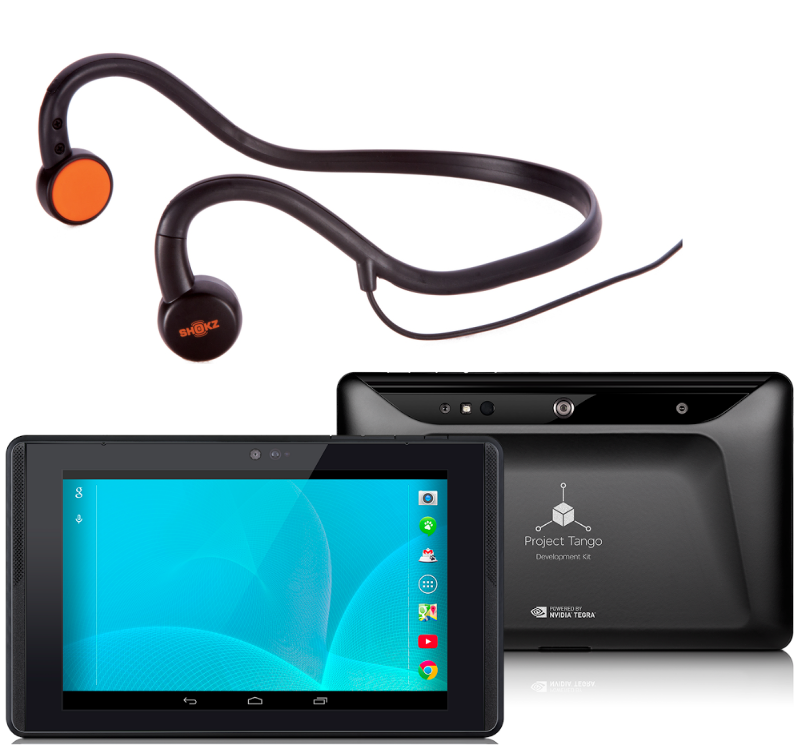
\includegraphics[width=0.3\textwidth]{figures/tango_headphone.png}
  \caption{A picture of the Tango device and the bone-conducting headset.}
  \label{fig:tango}
\end{figure}

We intend to use multiple feedback modes to provide the VI user with navigation and obstacle avoidance instructions. These modes are spatialised audio, voice prompts and vibration cues. However, for this paper, we only considered the spatialised audio mode in order to determine its effectiveness in conveying the tilt angle to a user.

A diagram of the entire system pipeline is shown in Figure~\ref{fig:pipeline}. Here, the arrows indicate the direction of the flow of information. When the user taps the Tango's screen, a new virtual target is generated and its coordinates are sent to the audio generation module, along with the Tango's current position and orientation. The audio generator then produces an audio tone based on the difference between these two sets of parameters and send it to the audio output channel that then plays it back to the user. The WiFi recording module is constantly monitoring the different parameter values of the Tango and target's position, as well as the system's output and records it to a remotely stored datafile. 

\begin{figure}
  \centering
  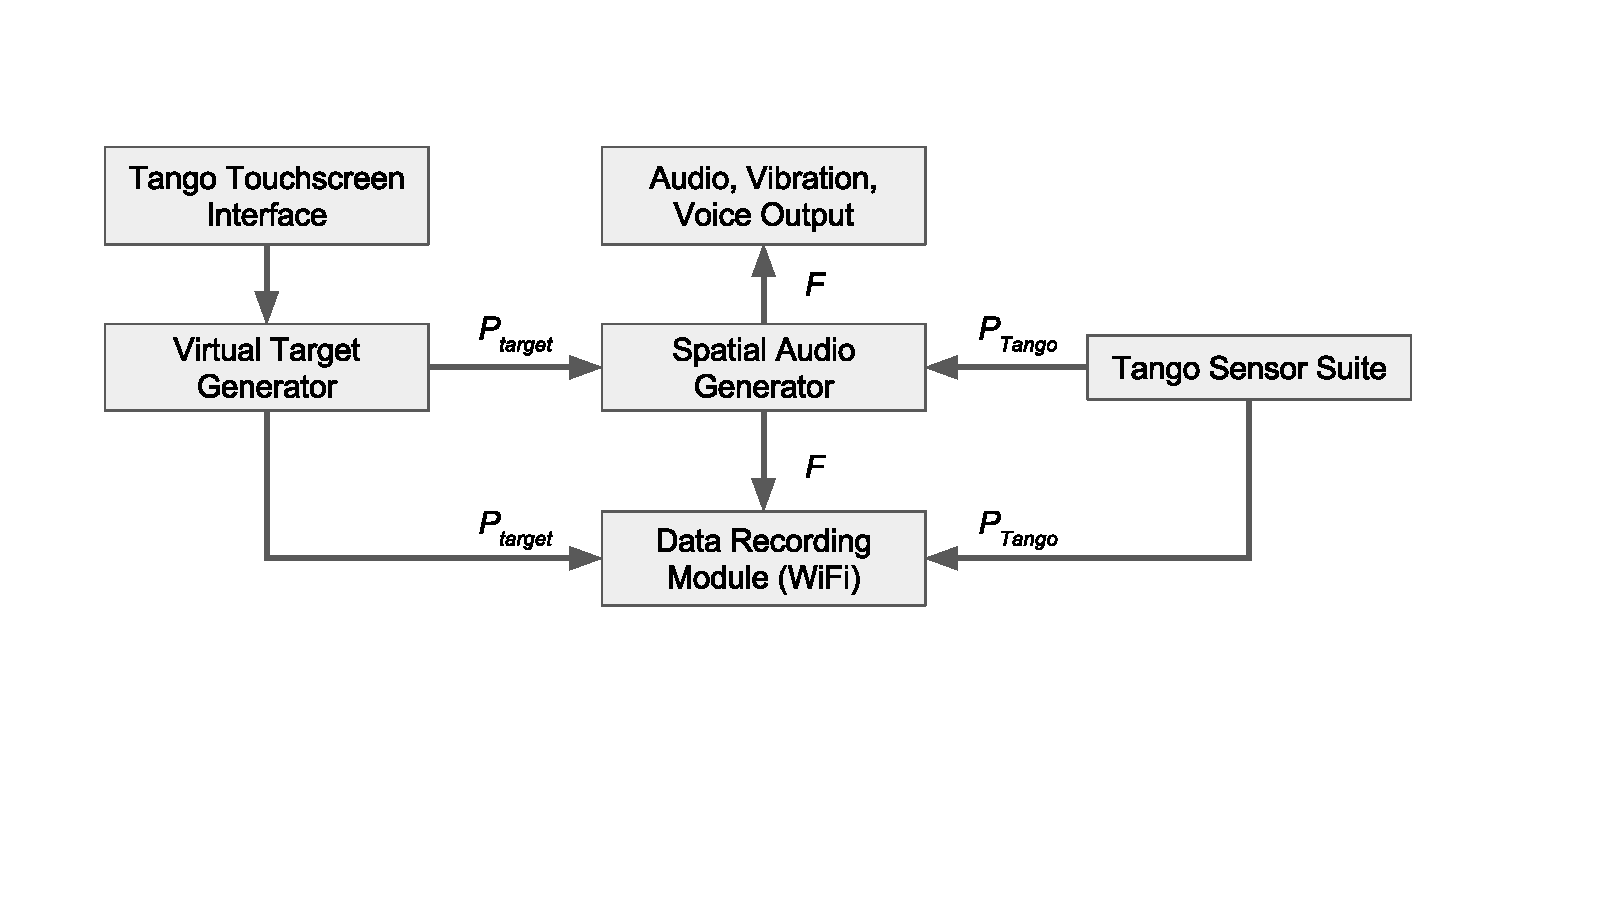
\includegraphics[width=0.45\textwidth]{figures/pipeline.pdf}
  \caption{A diagram of the individual system components and their communication pipelines. }
  \label{fig:pipeline}
\end{figure}

\section{Audio Interface}
\label{sec:interface}

For the series of experiments performed in this work, we only used the audio feedback mode to interface with the user. Here, the audio component is responsible for conveying the 2D position of a target on the vertical plane relative to the target in terms of pan and tilt angles. 

The audio being generated is a sinusoidal sound wave that is constantly generated and played to the user through bone-conducting headphones. We select a sinusoidal wave due to it being relatively simple to manipulate and analyse. %Furthermore, we opted to use an external, bone-conducting headset to play the audio to better simulate the use-case we are designing the system toward where our system will act as a supplementary navigation aid which does not interfere with their other senses; in particular their sense of hearing, which the VI tend to rely upon heavily. 

The audio is spatialised using and HRTF provided by a third-party open-source sound library. However, the audio is only spatialised in the pan dimension, while the tilt angle is conveyed by varying the pitch of the audio tone. We use this approach because the external set of bone-conducting headphones plays the sound through the user's cheekbones instead of their outer ears, bypassing the pennae of the ears which provide humans their ability to localise an elevated sound source~\cite{roffler1968factors, algazi2001elevation}, making it necessary to convey the tilt using another method. The difference between the target's angular position and the angular orientation of the Tango device are used to generate the audio navigation cues. %The argument has been made before in literature [CITE] that using this approach, as opposed to the head-mounted device approach, may be disorientating and unintuitive to a user. However, human beings are capable of externalising themselves and transfer their own frame of reference into an external object's and in our preliminary work, the users have not made any comments on the system being disorientating or confusing and after a brief training and familiarisation phase, has shown that they have no problem using the system and understanding the navigation cues. We would therefore argue that the head-mounted option conceptually offers no clear performance benefit over the hand-held exploration approach. 

\subsection{Pan Description}

The pan angle describes the angle which the user needs to rotate the camera vector around the $y$-axis, i.e. how far the target is to the left or right of the user. To communicate this user, we use a HRTF to add a spatial element to the audio tone that the system plays to the user, making the tone sound user like it is coming from the direction of the target. 

The HRTF functionality is implemented using the OpenAL library~\footnote{https://openal.org}~\cite{hiebert2005openal} to generate a sinusoidal sound wave based on the relative difference in the user and target's positions. We implement the library as a `black box' where the inputs are position values and it outputs a tone based on the the angle between the two position vectors and we implemented the same HRTF across all of the experiments we conducted.  

%OpenAL is able to generate a 3D spatial tone (pan, tilt and distance). However, we opted to only use it to convey the pan dimension and use other tools to convey the distance and tilt dimensions. We selected this approach partly because HRTFs commonly have difficulty communicating the tilt angle effectively, since its very reliant on the physical structure of the individual's ear and the high-frequency energy of the signal~\cite{roffler1968factors, algazi2001elevation}. 

%Furthermore, implementing other options for the distance and tilt dimensions grants us finer control over how they are communicated to the user.

\subsection{Tilt Description}

To communicate the tilt angle of the target, the system adjusts the emitted tone's pitch as a logarithmic function of the tilt angle, $\theta$, between the user's camera vector and the target's position. Here, a high pitch means the target is above the camera vector and the user should look up, whereas a low pitch means the target is below the camera vector and the user should look down. This high/low association scheme is selected, since humans naturally tend to associate high-pitched sounds with higher objects and lower-pitched noises with lower objects~\cite{pratt1930spatial}. We also opt for a logarithmic, octave-based gain function for the pitch, since an increase in octave provides a distinct perceptible change while keeping the timbre roughly similar~\cite{shepard1964circularity}.

We wish to determine what effect the gradient of the pitch gain function has on a user's performance; that is to say, does an increased rate of change in the pitch as a function of the tilt angle lead to an increased target acquisition rate, for example. For this we select three different pitch gain gradients, so-called \emph{lo}, \emph{med} and \emph{hi} high gain presets. To find these gradients, we set the maximum and minimum limits for the tilt and pitch angles. Furthermore, for the sake of consistency, each gradient is set to pass through the same pitch value at the \SI{0}{\radian} tilt angle.   

The neutral, \SI{0}{\radian}, position is set to be directly in front of the user and we limit the angles between $\pm$\SI[quotient-mode=fraction]{\pi / 2}{\radian}, requiring the system to be able to communicate angles within a range of \SI{\pi}{\radian}. Anything outside of this range implies that the target is behind the user. 

After practical tests with the Tango and the headphones, we set the neutral, on-target tone to a frequency of \SI{512}{\hertz} for its audibility. For the \emph{med} preset, we set the maximum and minimum pitches to be two octaves higher and lower than the neutral tone, giving limits of \SI{2048}{\hertz} and \SI{128}{\hertz} respectively. The \emph{lo} preset is set to one octave higher and lower than the neutral tone (\SI{1024}{\hertz} and \SI{256}{\hertz}) and the \emph{hi} to 3 octaves higher and lower (\SI{4096}{\hertz} and \SI{64}{\hertz} than the neutral tone. We selected these limits for practical reasons, given the fact that the bone conducting headphones we used have low volume gain at very high and low frequencies, making it difficult to hear. Figure~\ref{fig:pitch-preset-plot} shows the \emph{lo}, \emph{med} and \emph{hi} gain preset graphs.  

\begin{figure}
  \centering
  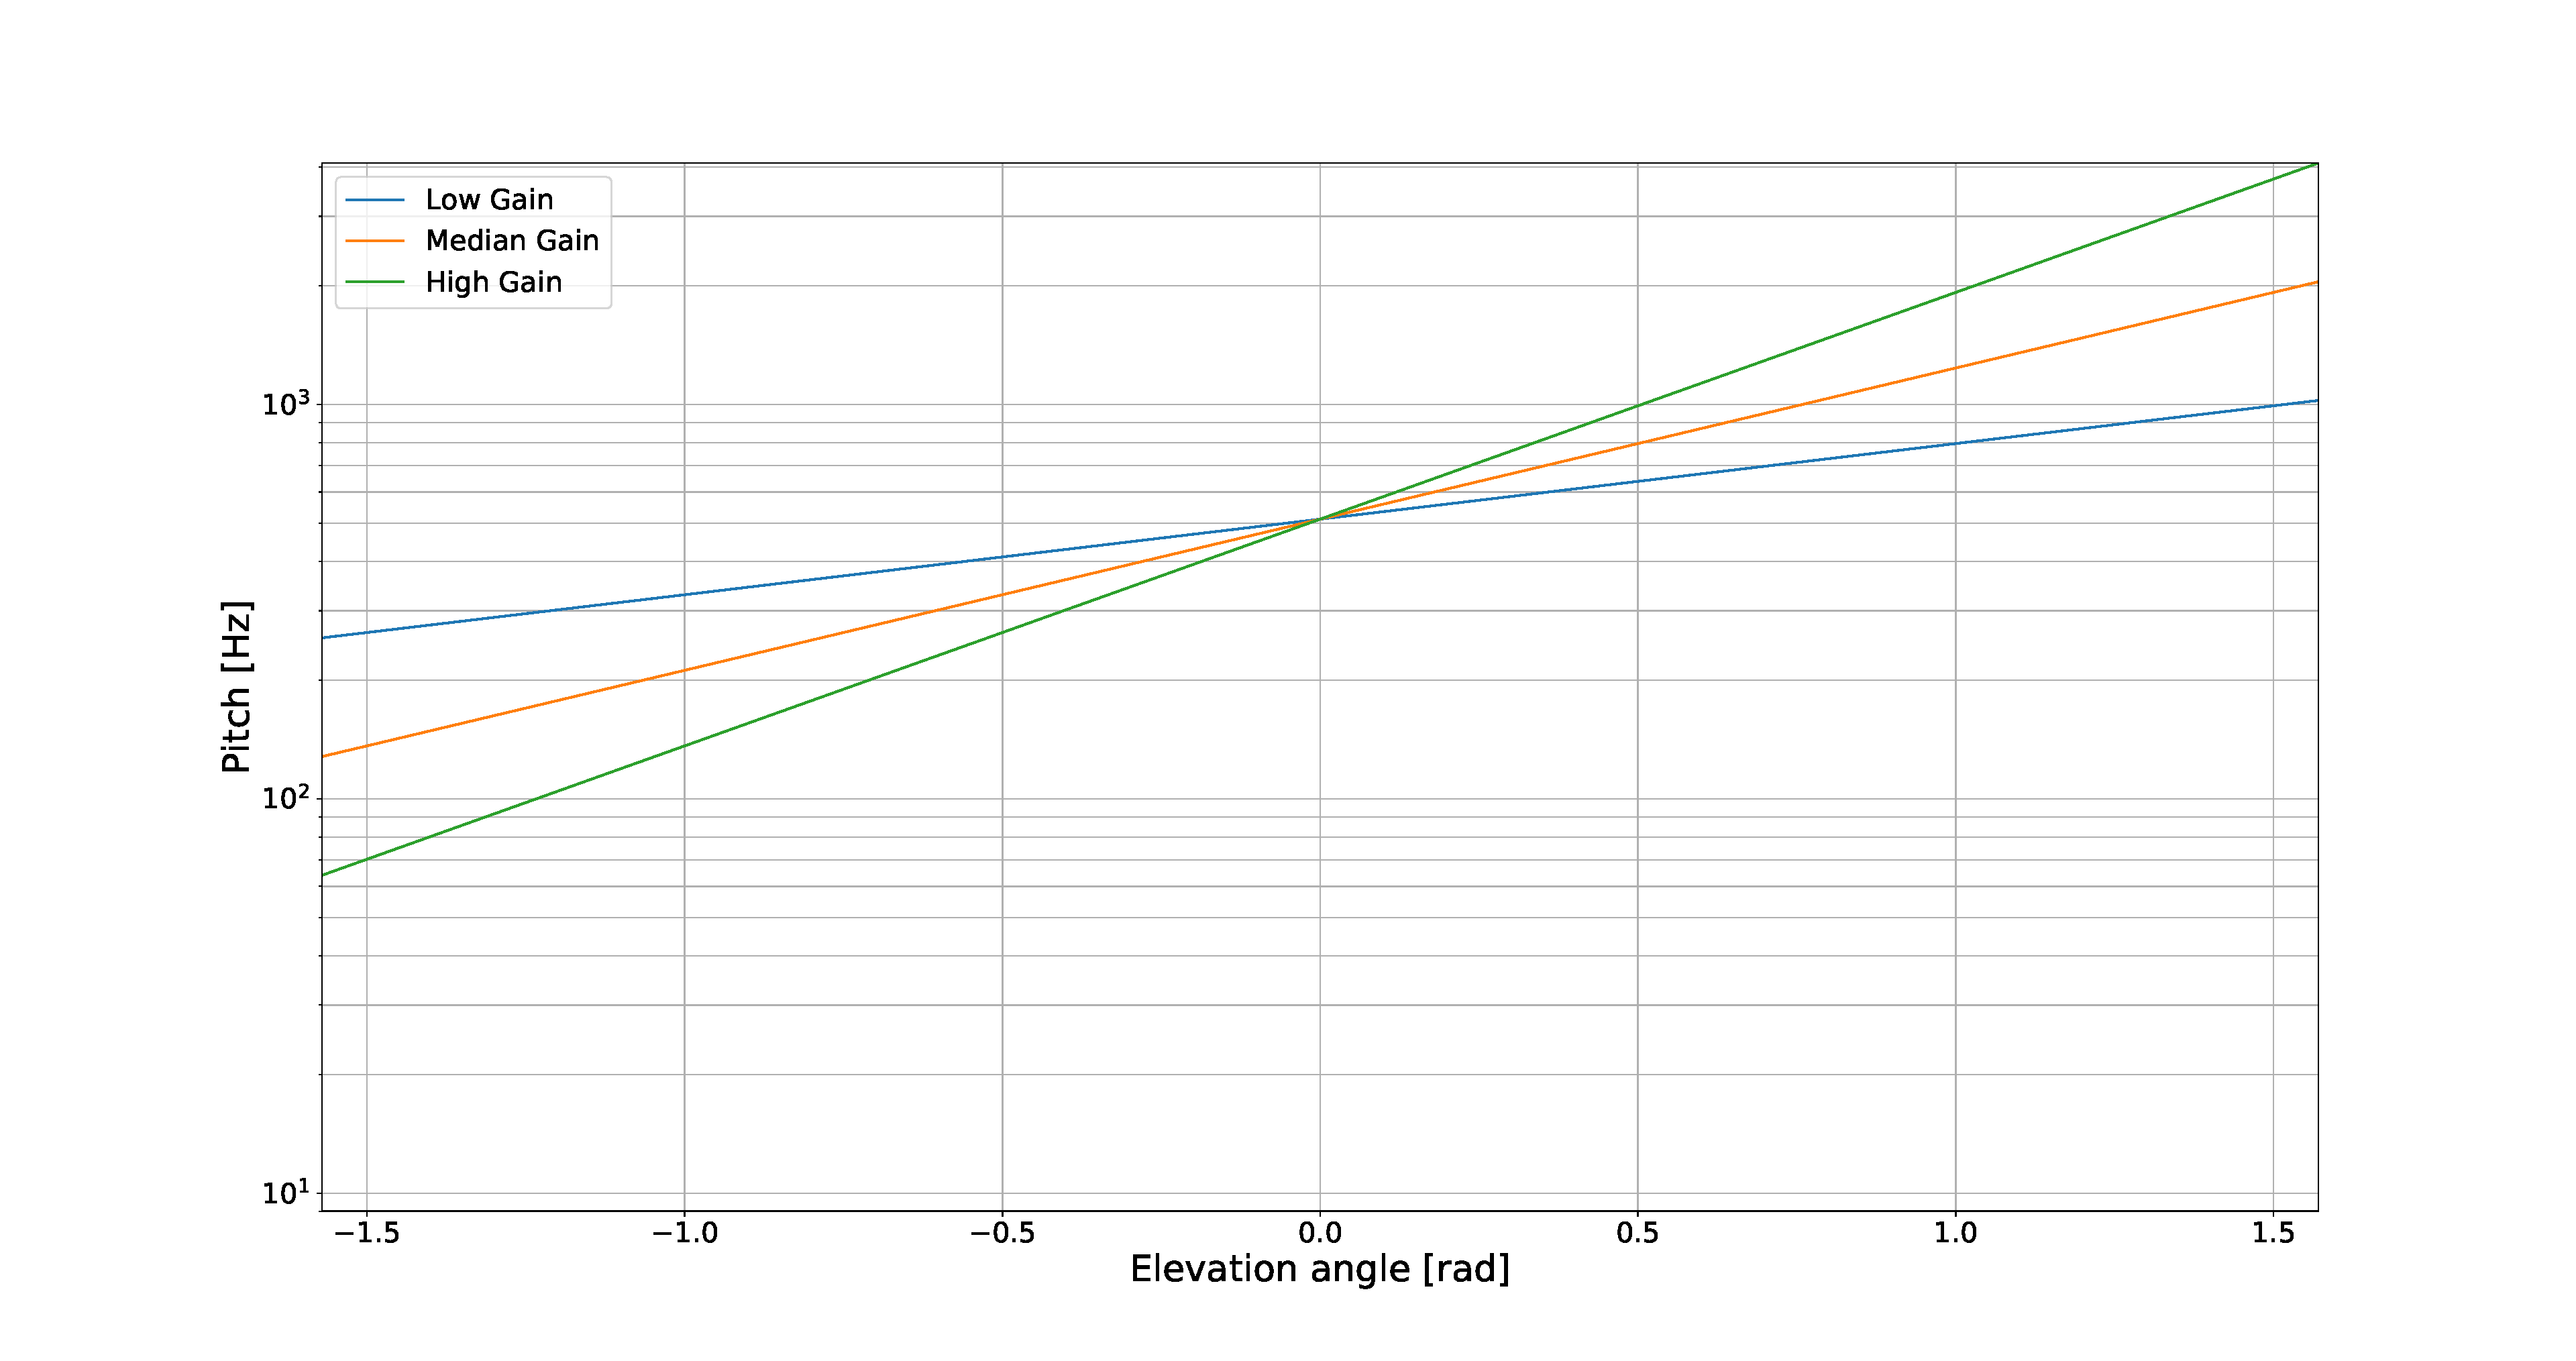
\includegraphics[width=0.5\textwidth]{figures/pitch_gradient.pdf}
  \caption{Plot depicting the different pitch gain preset functions.}
  \label{fig:pitch-preset-plot}
\end{figure}

\section{Experiments}
\label{sec:experiments}

To determine how effective the individual feedback modes of our HMI is at directing a user to perform a given task, we performed a set of experiments with blindfolded users using a limited set of the feedback modes. %The reason for only experimenting with one or two modes together is to simplify the experiment procedure and incrementally build up our knowledge of the interactions between the user and the feedback mode so that we can eventually integrate all of the feedback modes into a single implementation and perform an optimal set of experiments that will provide us with all of the important data that we require. 

In this case, we experimented with the spatialised sound feedback mode; that is to say we determined how effective a spatial tone, with varying pitch, is at directing a user to pan and tilt a camera to find a target. Furthermore, we also carried out a set of pre-screening experiments to determine each subject's hearing characteristics. %The following sections will discuss all of these experiments and their objectives in detail. 

We plan to use the results from the experiments we performed to better understand how the users respond to different settings for the feedback stimuli mentioned earlier, in order to improve and optimise the behaviour of the feedback modes.

%\subsection{Experiment Objectives}

%Every subject was asked to participate in 4 different experiments: the first three were pre-screening experiments to evaluate the subjects' hearing characteristics and the last to determine how effective our HMI's spatial sound is at controlling a subject's pan and tilt. Furthermore, we wish to determine how the different values of this spatial sound affects a subject's performance. 

%The hearing characteristics we wished to determine were the subjects' spatial awareness, tone limits and tone discrimination capability. For the spatial sound experiment we wish to determine how quickly each subject can find their target's, what each subject's target search strategy is as well as how the different feedback parameter values affect these performances. 

\subsection{Experimental Procedure}

For the experiments we used 42 sighted, but blindfolded volunteers and had them perform a series of experiments using our system and a pair of bone-conducting headphones. The subjects were recruited on a volunteer-basis and consisted of a diverse group of undergraduate students with ages ranging between 18 and 27 years, with the 10 being male and 32 female. The subjects also reported having no significant sight or hearing issues or any other major disability. 

The subjects were asked to participate in 3 experiments, each of which are discussed here. The first 2 experiments were performed to determine each subject's hearing characteristics and capabilities to provide some context to the results generated during the 3rd and final target-search experiment. These characterisation experiments were performed to check if the subjects had any pre-existing biases in the modes or dimensions we were going to perform our target search experiment in. 

\subsection{Subject Characterisation}

\subsubsection{Spatial Awareness}

In this experiment, we evaluate a subject's ability to determine the direction a sound is coming from. To do this, we play a \SI{512}{\hertz} sinusoidal tone to the subject through the headphones and apply an HRTF to it to make it sound like its coming from either the left or right of the subject. The subject must then select whether the sound is coming from the left or right. The longer the experiment is run, the closer the source moves to the centre-front of the subject, making it more difficult to localise the sound source. 

For this progressive increase in difficulty, a 2-up, 1-down step process is used, meaning that for every 2 correct answers, the distance to the centre halves, making the process harder. Conversely, it becomes easier for each incorrect answer by doubling the sound source's distance from the centre. We also use 2 different step sequences, one starting at a large distance (\SI{2}{\m}) from the user and the other at the minimum distance (approximately \SI{3}{\cm}), giving an `easy' and `hard' step respectively. The terminating condition for the experiment is when the 2 step sequences are within 2 step ranges, i.e. if one distance is less four-times bigger or smaller than the other, of each other for 3 consecutive guesses. This gives a distance band within which the subject is capable of localising the sound source. Each subject performs this experiment three times. 

\subsubsection{Pitch Discrimination}

In this experiment, we determine a subject's ability to tell tones with different frequencies apart, i.e. how well can they tell if a tone is high or low pitched? Here we play 2 tones to the subjects, one after the other, with the second being higher or lower-pitched than the first tone. The subjects are then asked to select whether the second tone was higher or lower-pitched than the first tone.

The first tone was randomly generated by the app and the second tone was generated by adding or subtracting the difference from the first tone. This difference determines the difficulty and is based on an exponential function, $f(n) = n^2$, where $n$ is increased or decreased to adjust the differentiation difficulty. 

As with the spatial experiment, a 2-up, 1-down step process is used: for every 2 consecutive correct answers, the pitch difference between the two tones are halved, increasing the difficulty, and the difference is doubled, i.e $n$ is incremented by 1, for every incorrect answer, making the tones easier to differentiate. Two step sequences are again used here, one starting with a large pitch difference (\SI{512}{\hertz}) between the tones and the other with a small difference (\SI{2}{\hertz}). The termination condition is when the two step sequences are within one octave of each other for 3 consecutive answers. Each subject performed this experiment twice. 

%\textbf{Tone Limit Experiment}: We determined the subjects' tone limits as a final experiment before they took part in the  main, target-finding experiment. We did this by playing a single tone that increases in pitch as time progresses. The subject was then asked to click a button as soon as he/she started hearing a tone and to click the button again when the tone became inaudible. The subject was then asked to repeat the process 6 times, but the tone direction was reversed after each run, meaning that the tone either started high and went low or started low and went high. 

\subsection{Target Search}

\subsubsection{Task}

The final experiment is the main one and will answer the question we are most interested in: how well does a spatial tone with varying pitch direct a user to look in a specific direction, and how do the parameters of this tone affect the user's performance in this task? %To answer this question, we use two different metrics to compare the three different pitch gradient settings: the accuracy and the target search time. The methods we use are described here. 

For this experiment, the subject is blindfolded and given a Tango device running an app written specifically for this experiment. When started, a set of virtual targets are presented one at a time to the subject on the Tango device. Then, depending on the direction the subject is currently pointing the camera relative to the target's position, the Tango generates and plays a tone via the bone-conducting headphones to indicate the pan and tilt angle adjustment the subject needs to make the camera point to the target. These instructions are spatialised tones with varying pitch: an HRTF indicates whether the target is to the left or the right and the pitch indicates whether the subject should be looking up (high pitch) or down (low pitch) to find the target. 

The distance between the subject and the target is not considered here. Therefore, the targets are generated on the vertical plane at a constant distance from the subject, in this case \SI{2}{\m}. Throughout the experiment, various parameters of the target and the subject are recorded and streamed in real-time to a laptop computer via a WiFi connection.

Once the subject has pointed the camera toward the target, the HRTF centres the tone in front of the subject with a neutral pitch of \SI{512}{\hertz}, which we use as the `on-target' pitch for all of our experiments.  However, the subject have to decide for themselves whether they truly are looking at the target and tap the screen to indicate the direction they believe the target is in. At this point a new target is presented to the subject which they have to search for again. 

28 targets are presented to each subject per round. The positions of these targets are randomly generated and are equally spread across the 4 quadrants on the vertical plane to prevent a lumping of targets at one location. After every round of experiments, the parameters controlling the tone's behaviour were adjusted. In this case, the rate of change of the tone's pitch was adjusted to make the pitch increase at a lower or higher rate as a function of the tilt angle between the target and the subject's current gaze direction. This was done to see whether, for example, a more rapid increase in pitch will help the subject find the target faster. 

The subjects were given a few minutes without a blindfold prior to the experiment started where they could familiarise themselves with the system where they could confirm the target's location with their own eyes.

\subsubsection{Metrics}

We use two different metrics to compare the three different pitch gradient settings: the accuracy and the search time. 

The accuracy is given as the difference between the Tango's angular orientation at the time the subject confirmed they were on target, and the target's actual angular position. We separate the results from the tile and pan dimensions in order to see how the different pitch gradients affect a subject's pointing accuracy. 

%The performance between the three difference pitch gradient configurations can be compared using different metrics. The previous sections established the difference in accuracy between the configurations.

We also compare the performance of the three pitch gradient settings in terms of the time it took each subject to find a target. However, since each subject was presented with a different, randomly generated set of targets, a direct time comparison is impossible. Therefore, for this analysis, we opt to use Fitts's Law~\cite{fitts1954information} which states that there is a logarithmic relation between the time it takes to find a target and the index of difficulty of the target (the ratio between the distance to the target and its width). It also gives us a so-called `index of performance' that we can use as a metric to compare the results between the three configurations. Fitts's Law is given in Equation~\ref{eq:fitts-base}. 

\begin{equation}
  \label{eq:fitts-base}
  t = a + b\log_2\left(\frac{d}{w} + 1\right)
\end{equation}

Here, $t$ is the time it takes to find the target and $d$ is the distance between the two subsequent targets' centre points, while $w$ is the width of the target and $a$ and $b$ are constants determined through regression.

Fitts's Law uses the target's width as a parameter in its index of difficulty. However, our targets do not have a width, which means we have to use a modified form of Equation~\ref{eq:fitts-base} that uses an effective width, $w_e$, as a parameter instead. Using this parameter was originally proposed by \citeauthor{mackenzie1992fitts}~\cite{mackenzie1992fitts} in order to provide more accurate results when the process contains noise and uncertainties. In our case, the noise is introduced by the subjects not selecting the target at a constant distance from the target's centre. 

$w_e$ is given by 

\[
  w_e = \sqrt{2\pi e}\sigma = 4.133\sigma
\]

where $\sigma$ is the standard deviation in the error data, taken as the difference in Euclidian distance between the subjects' target selections and the targets' actual positions. This results in the modified form of Fitts's Law, given in Equation~\ref{eq:fitts-simple}.

\begin{equation}
  \label{eq:fitts-simple}
  t = a + b\log_2\left(\frac{d}{4.133\sigma} + 1\right) = a + b ID
\end{equation}

Here $ID$ is shorthand for the Index of Difficulty. Fitts's index of performance~\cite[p.~390]{fitts1954information}, $IP$, can then be calculated using the relation from Equation~\ref{eq:fitts-performance}. 

\begin{equation}
  \label{eq:fitts-performance}
  IP = \frac{ID}{t}
\end{equation}

\section{Results}
\label{sec:results}

\subsection{Subject Characterisation}

Figure~\ref{fig:location-guesses} shows the results for the spatial awareness experiment, where the subjects had to determine the location of the sound they were played. 

\begin{figure}
  \centering
  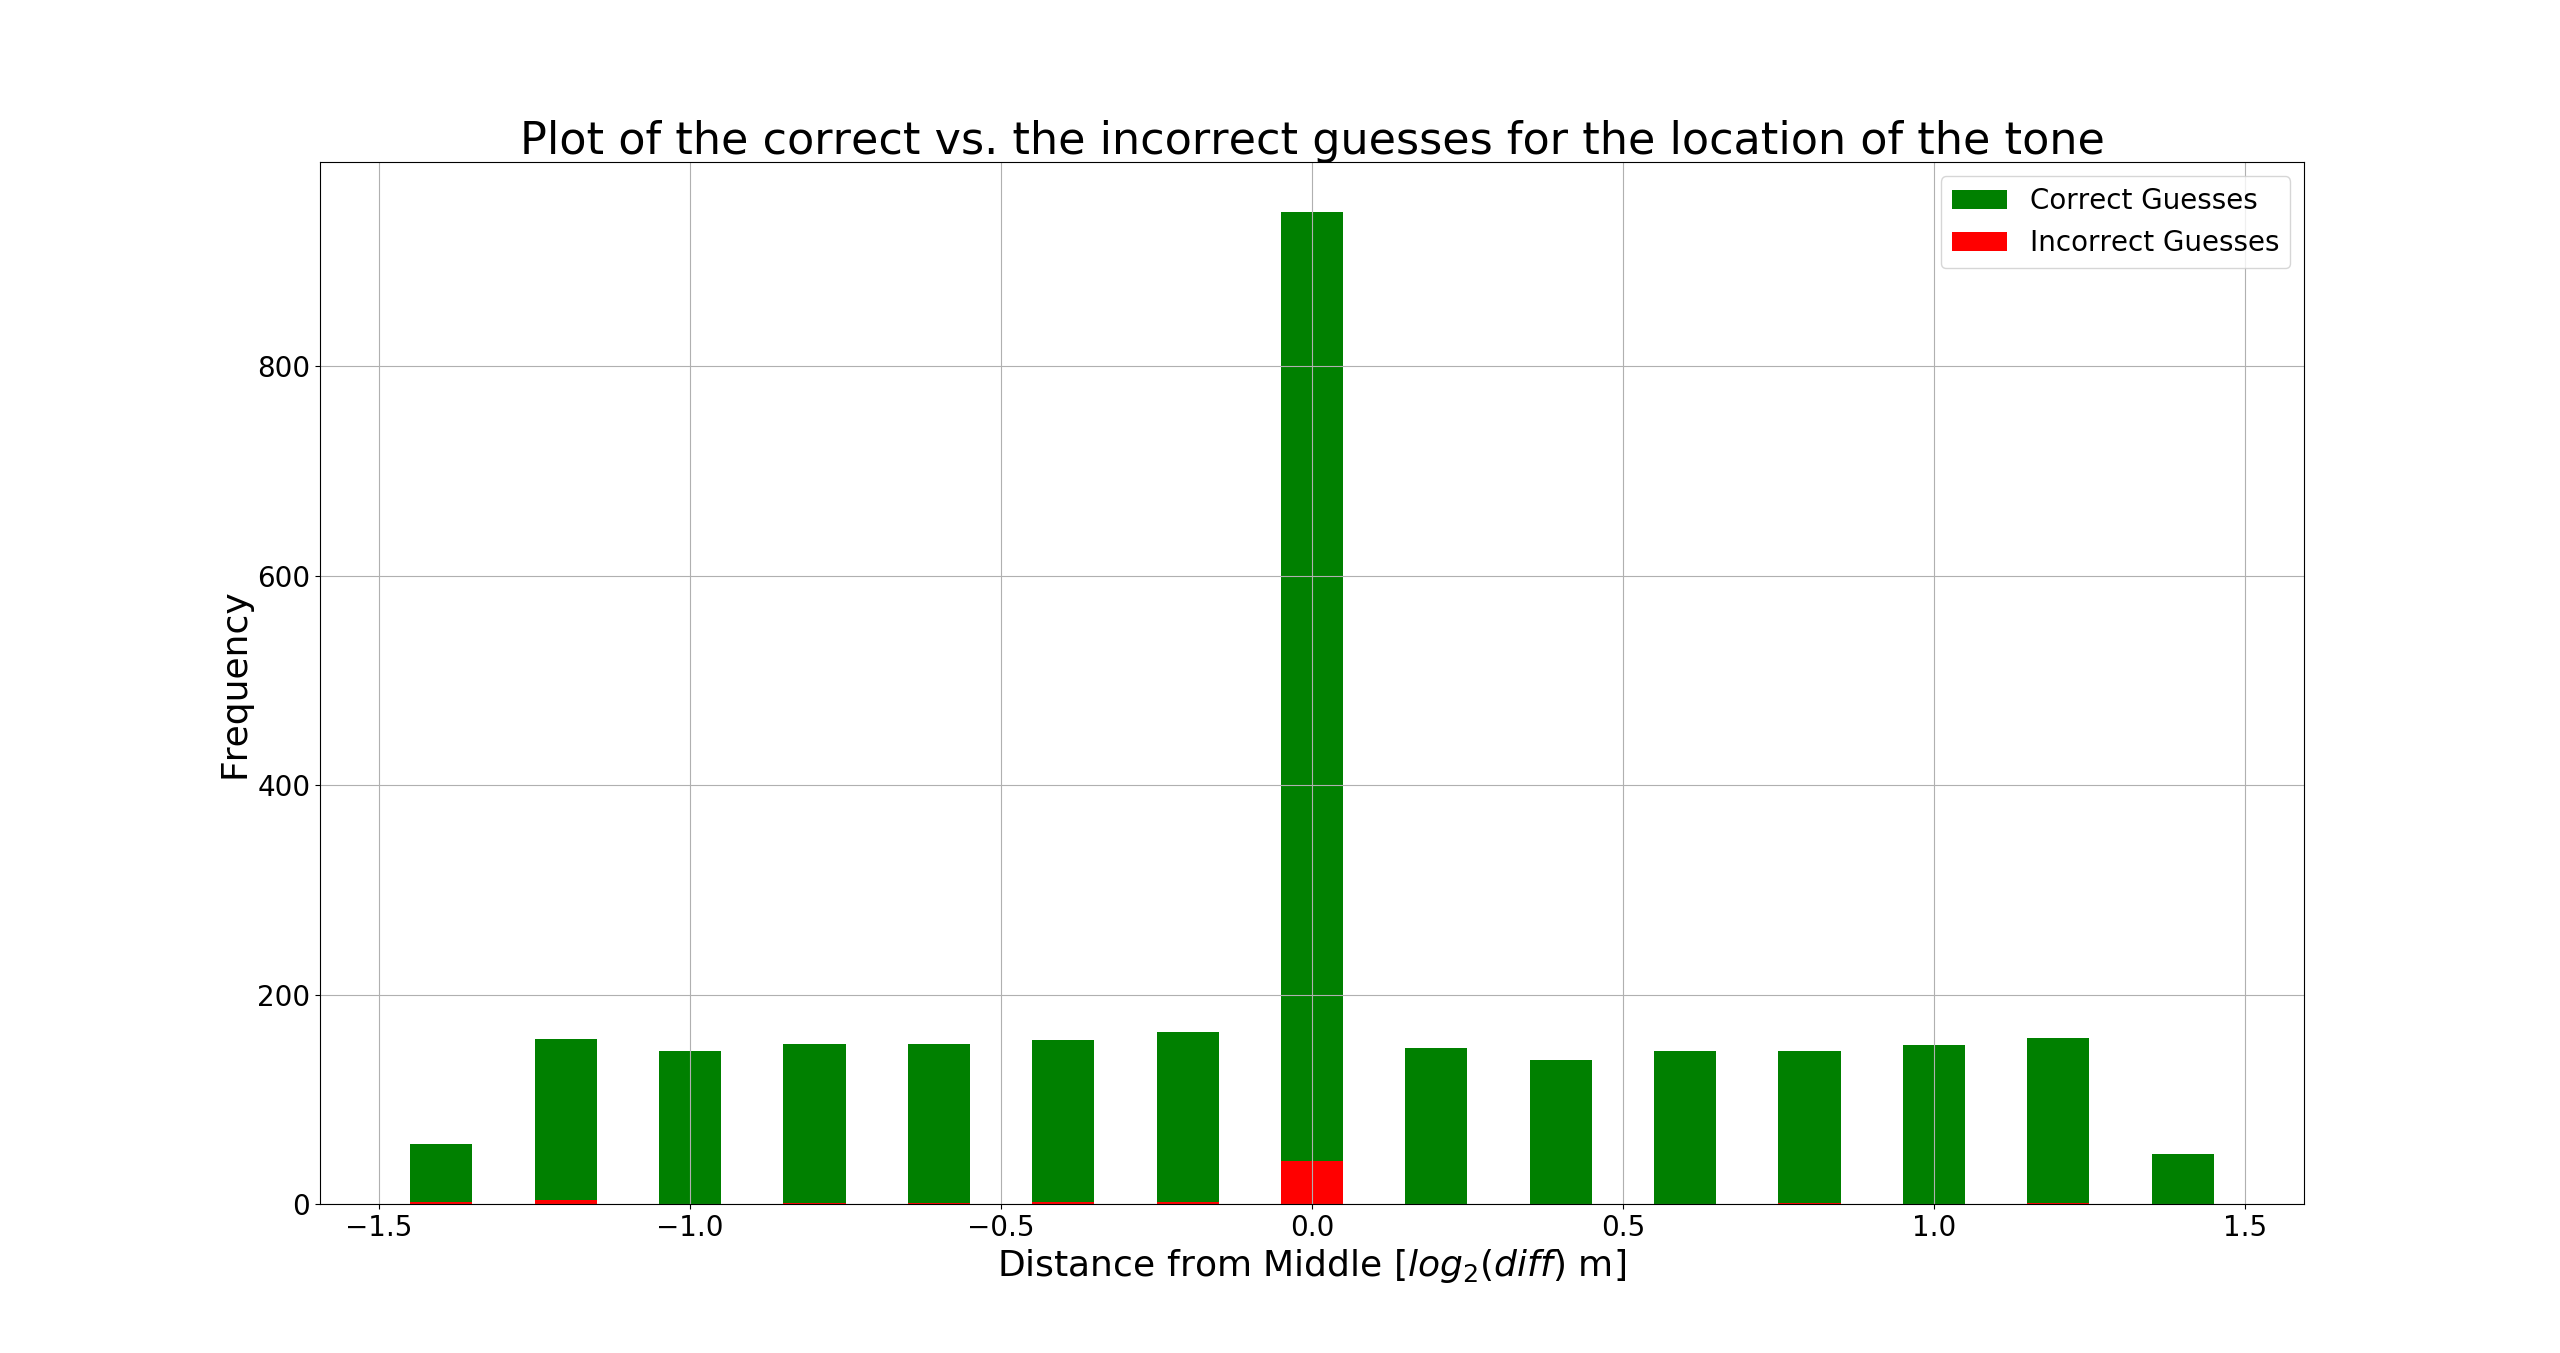
\includegraphics[width=0.5\textwidth]{figures/location_guesses.png}
  \caption{A bar plot showing the subjects' guesses about the tones' locations.}
  \label{fig:location-guesses}
\end{figure}

With the relatively low number of red, incorrect guesses, we see that the subjects were far more successful in correctly guessing the location of the sound source. This is further supported by the large number of samples at the minimum difference level of \SI{0.03125}{\m}, indicating that the subjects reached this level more frequently and consistently. Here we can see that the subjects had little problem localising the left-right direction of a sound source. 

These results are in line with what we expected and is supported by literature which indicates that humans are very adept at localising the location of a sound source and this ability was apparent for HRTF-generated pan location. 

The results recorded during the pitch discrimination experiment are shown in Figure~\ref{fig:tone-guesses} where a bar plot is used to show the frequency of correct guesses versus the incorrect guesses for each tone difference level. 

\begin{figure}
  \centering
  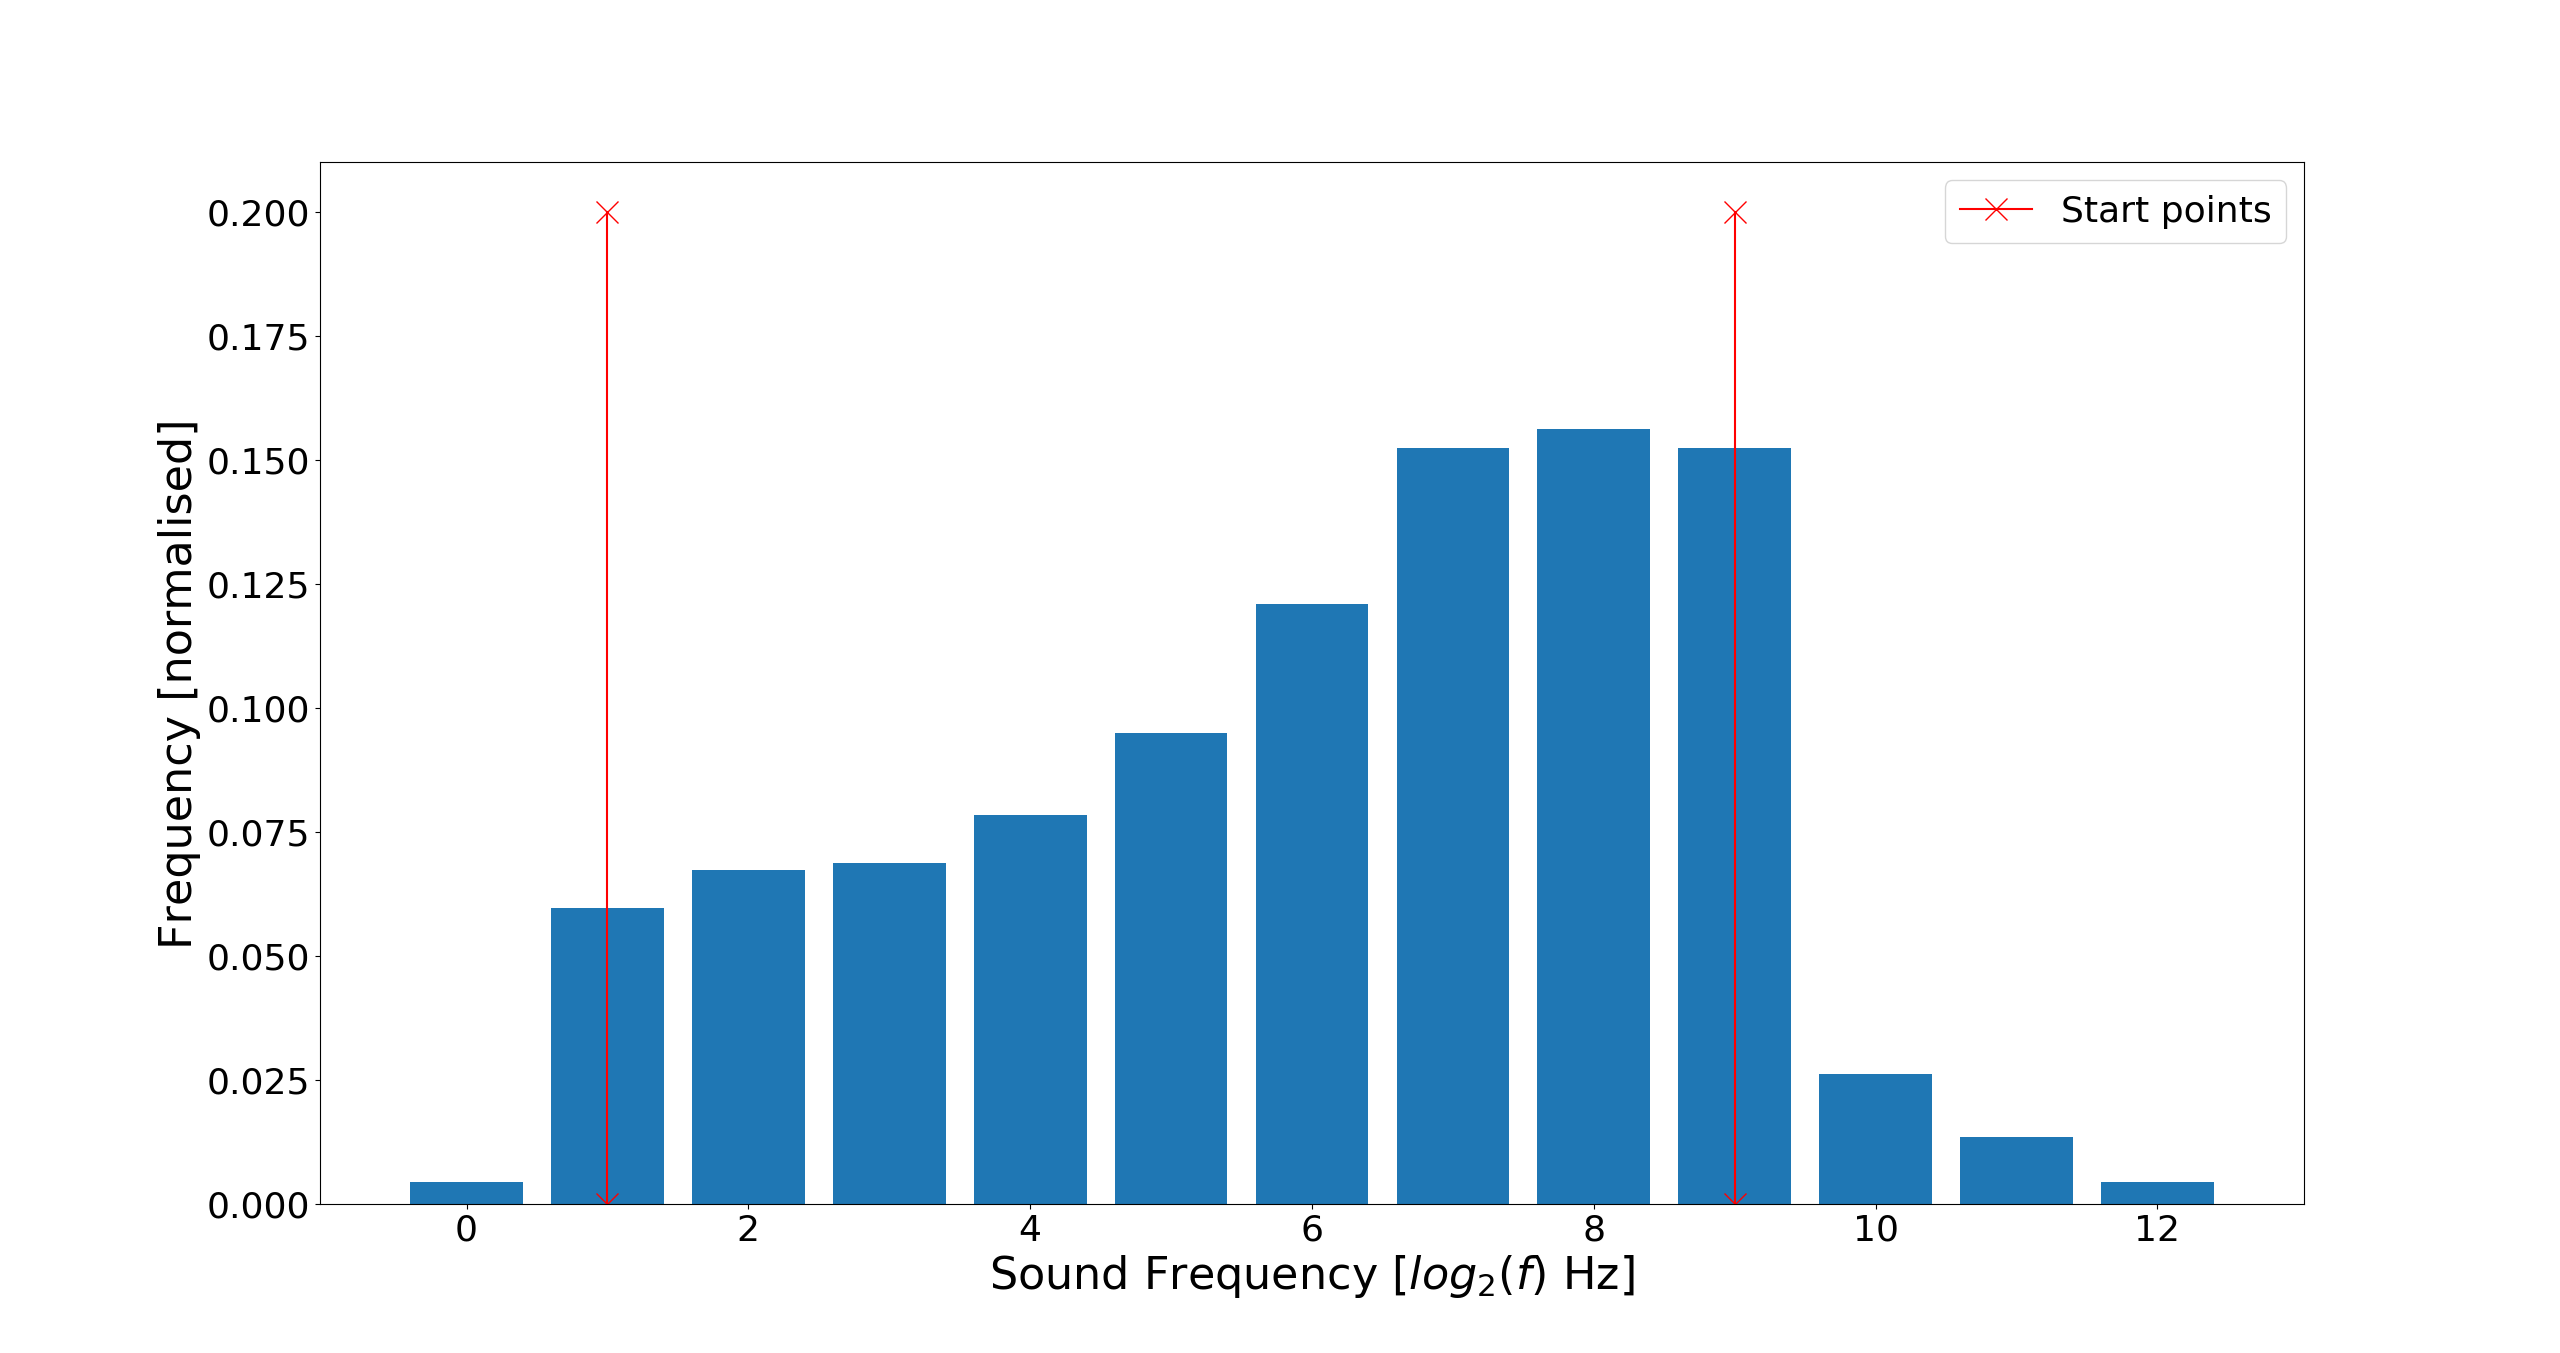
\includegraphics[width=0.5\textwidth]{figures/tone_guesses.png}
  \caption{A bar plot showing the subjects' guesses about the tone differences.}
  \label{fig:tone-guesses}
\end{figure}

As one might expect, the number of samples at the extreme, larger tone differences are significantly higher than for the smaller differences, where around 80\% of the respondents' correct answers were given at a difference of \SI{16}{\hertz} or more, with the reason being that it is easier to discriminate between two tones with a large tone difference. The number of incorrect guesses in this interval makes up approximately 50\% of the total number of incorrect guesses. For frequencies less than \SI{16}{\hertz}, the number of correct guesses drops down to 20\% of the total correct guesses, while the amount of incorrect guesses remain around 50\% of the total incorrect guesses made.

This indicates that our subjects' incorrect answers are fairly consistent across the frequency spectrum, but correct tonal discrimination is far more likely to occur with frequency differences larger than \SI{16}{\hertz}.  

%These results are in line with what one might expect, where it becomes increasingly difficult to differentiate between two tones with a small difference for a typical user. However, these results are useful for our research when we begin implementing autonomous adaptation capabilities into our system. 

\subsection{Target Search}

\subsubsection{Tilt Results}

Figure~\ref{fig:tilt-err} shows the results recorded during the target search experiment for the tilt dimension. Plots are presented for each of the three pitch gain gradients, i.e. \emph{lo}, \emph{med} and \emph{hi}. Scatter plots of the subjects' guesses of where the targets are vs. the targets' actual locations are given, along with linear regression plots to show the correlation between the data sets. A histogram is also given along with each plot to help the reader visualise the spread of the error data. Finally, a set of box-plots are given in Figure~\ref{fig:tilt-boxplots} to convey the average angular error between the subjects' guesses and the targets' true positions.

The results are summarised in Table~\ref{tab:tilt-results}.

\begin{figure}
  \centering
  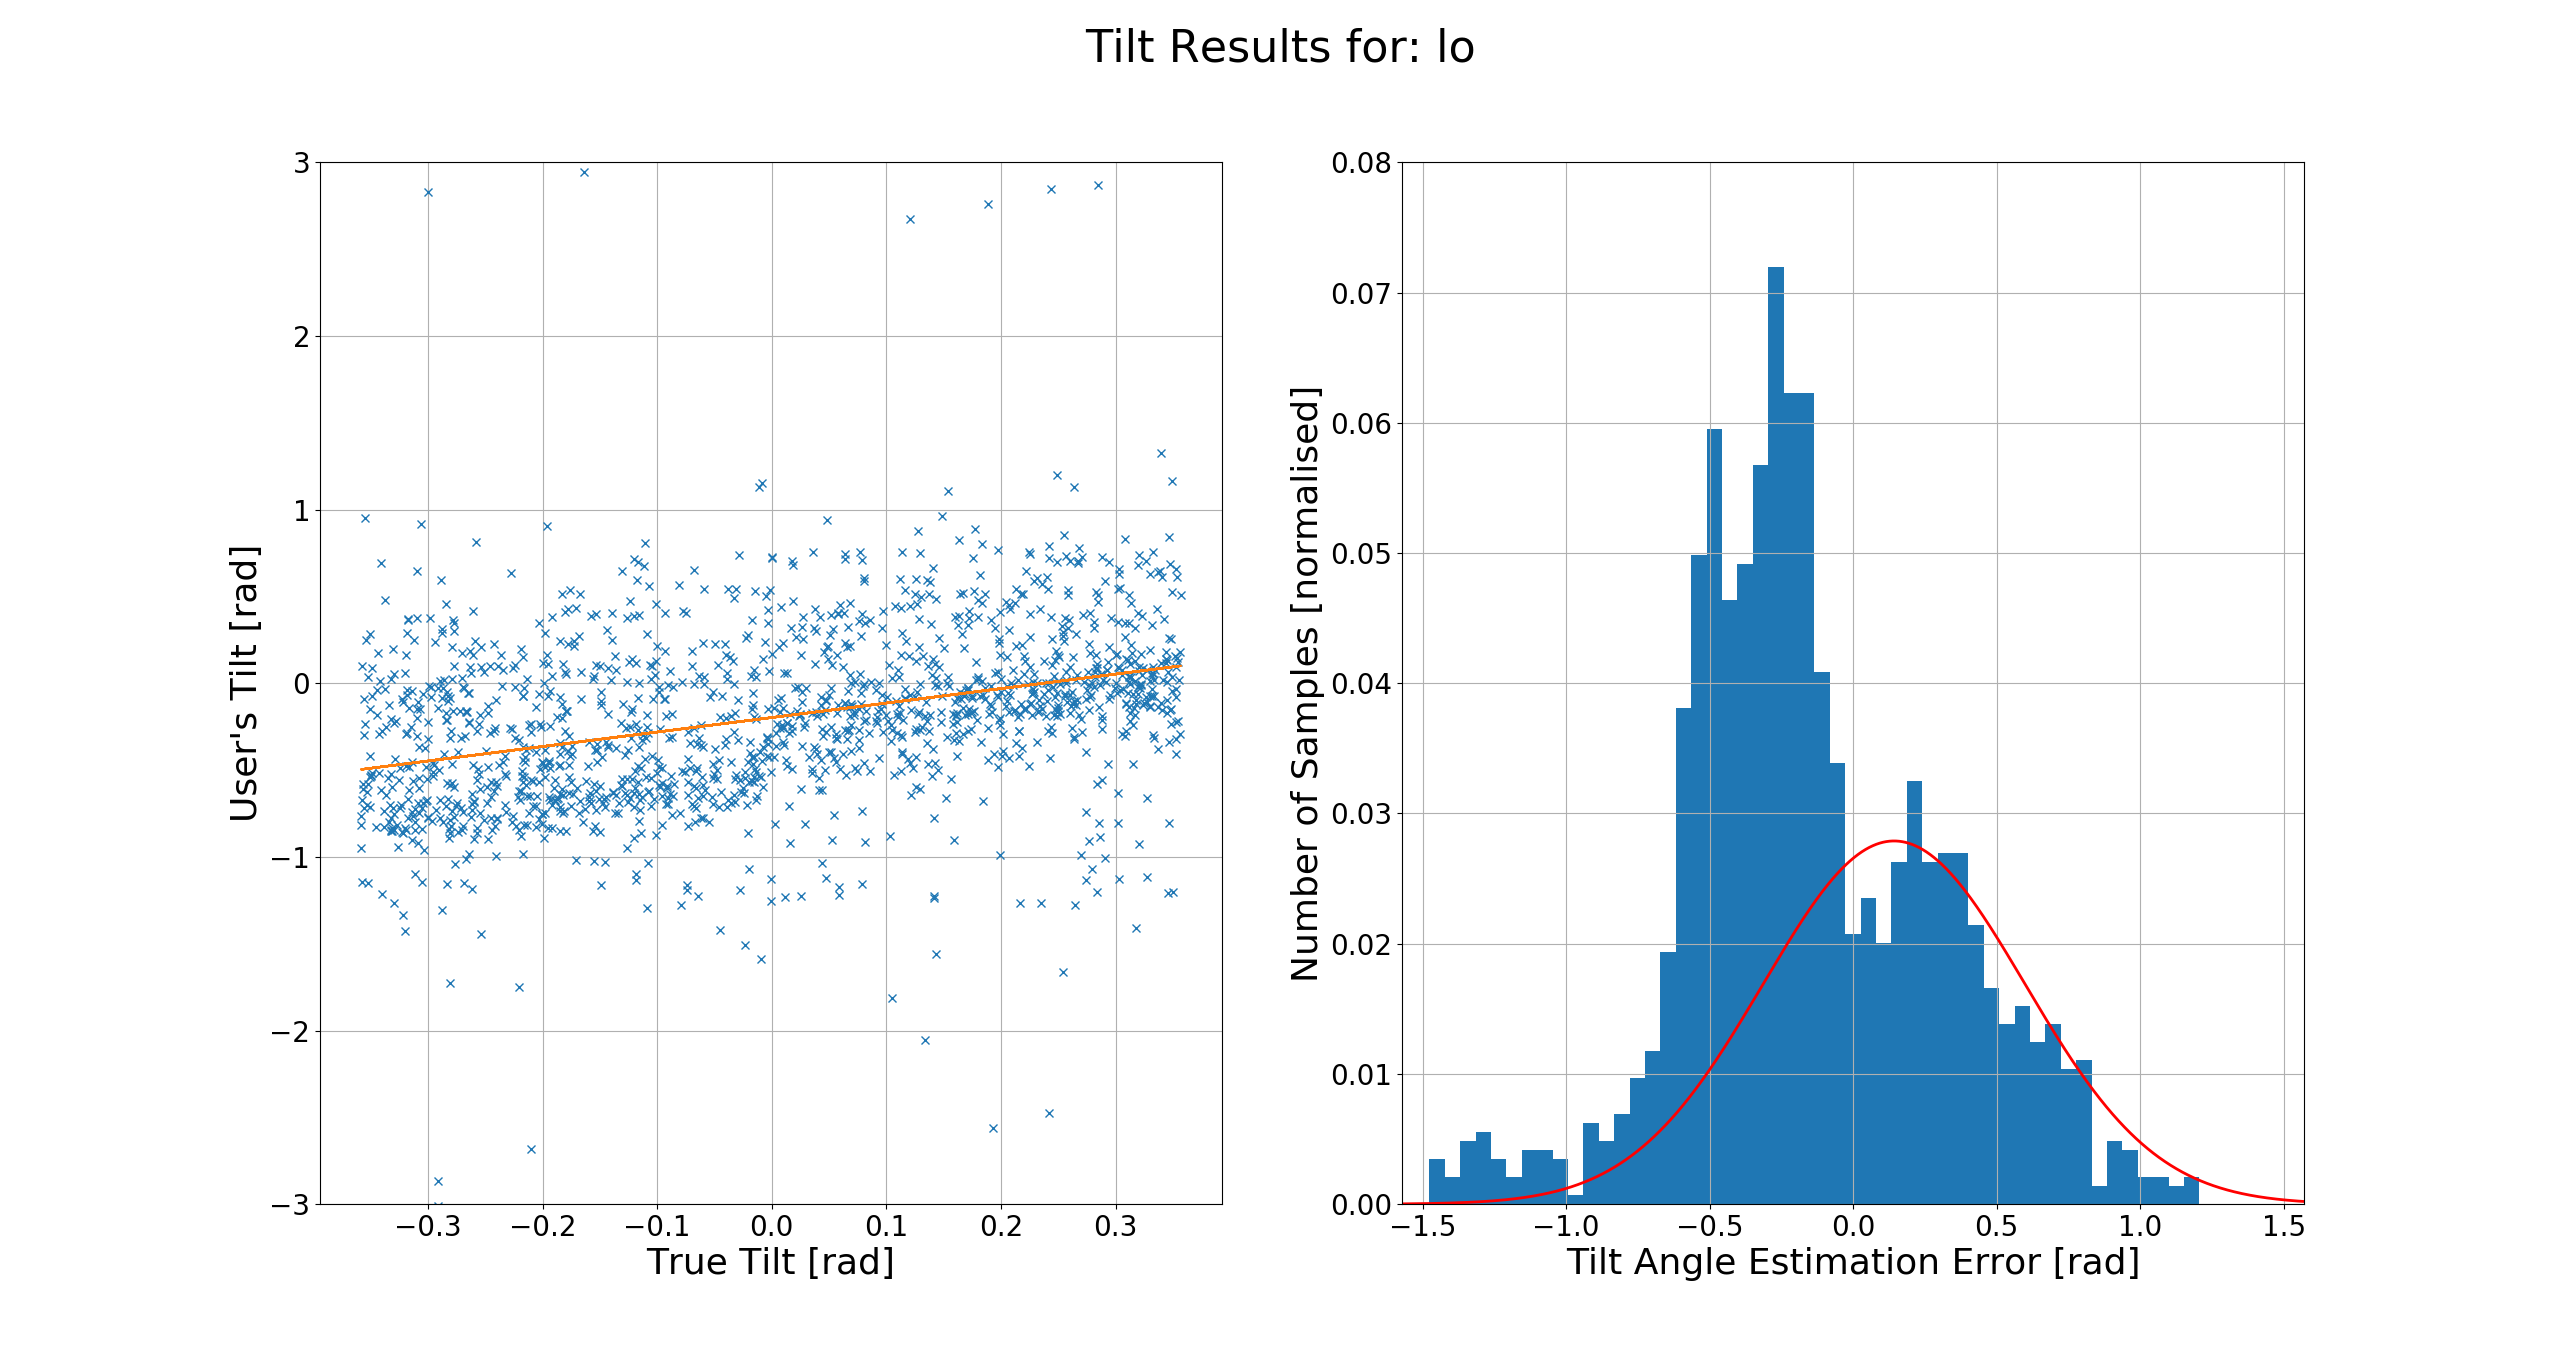
\includegraphics[width=0.5\textwidth]{figures/tilt_err_lo.png}
  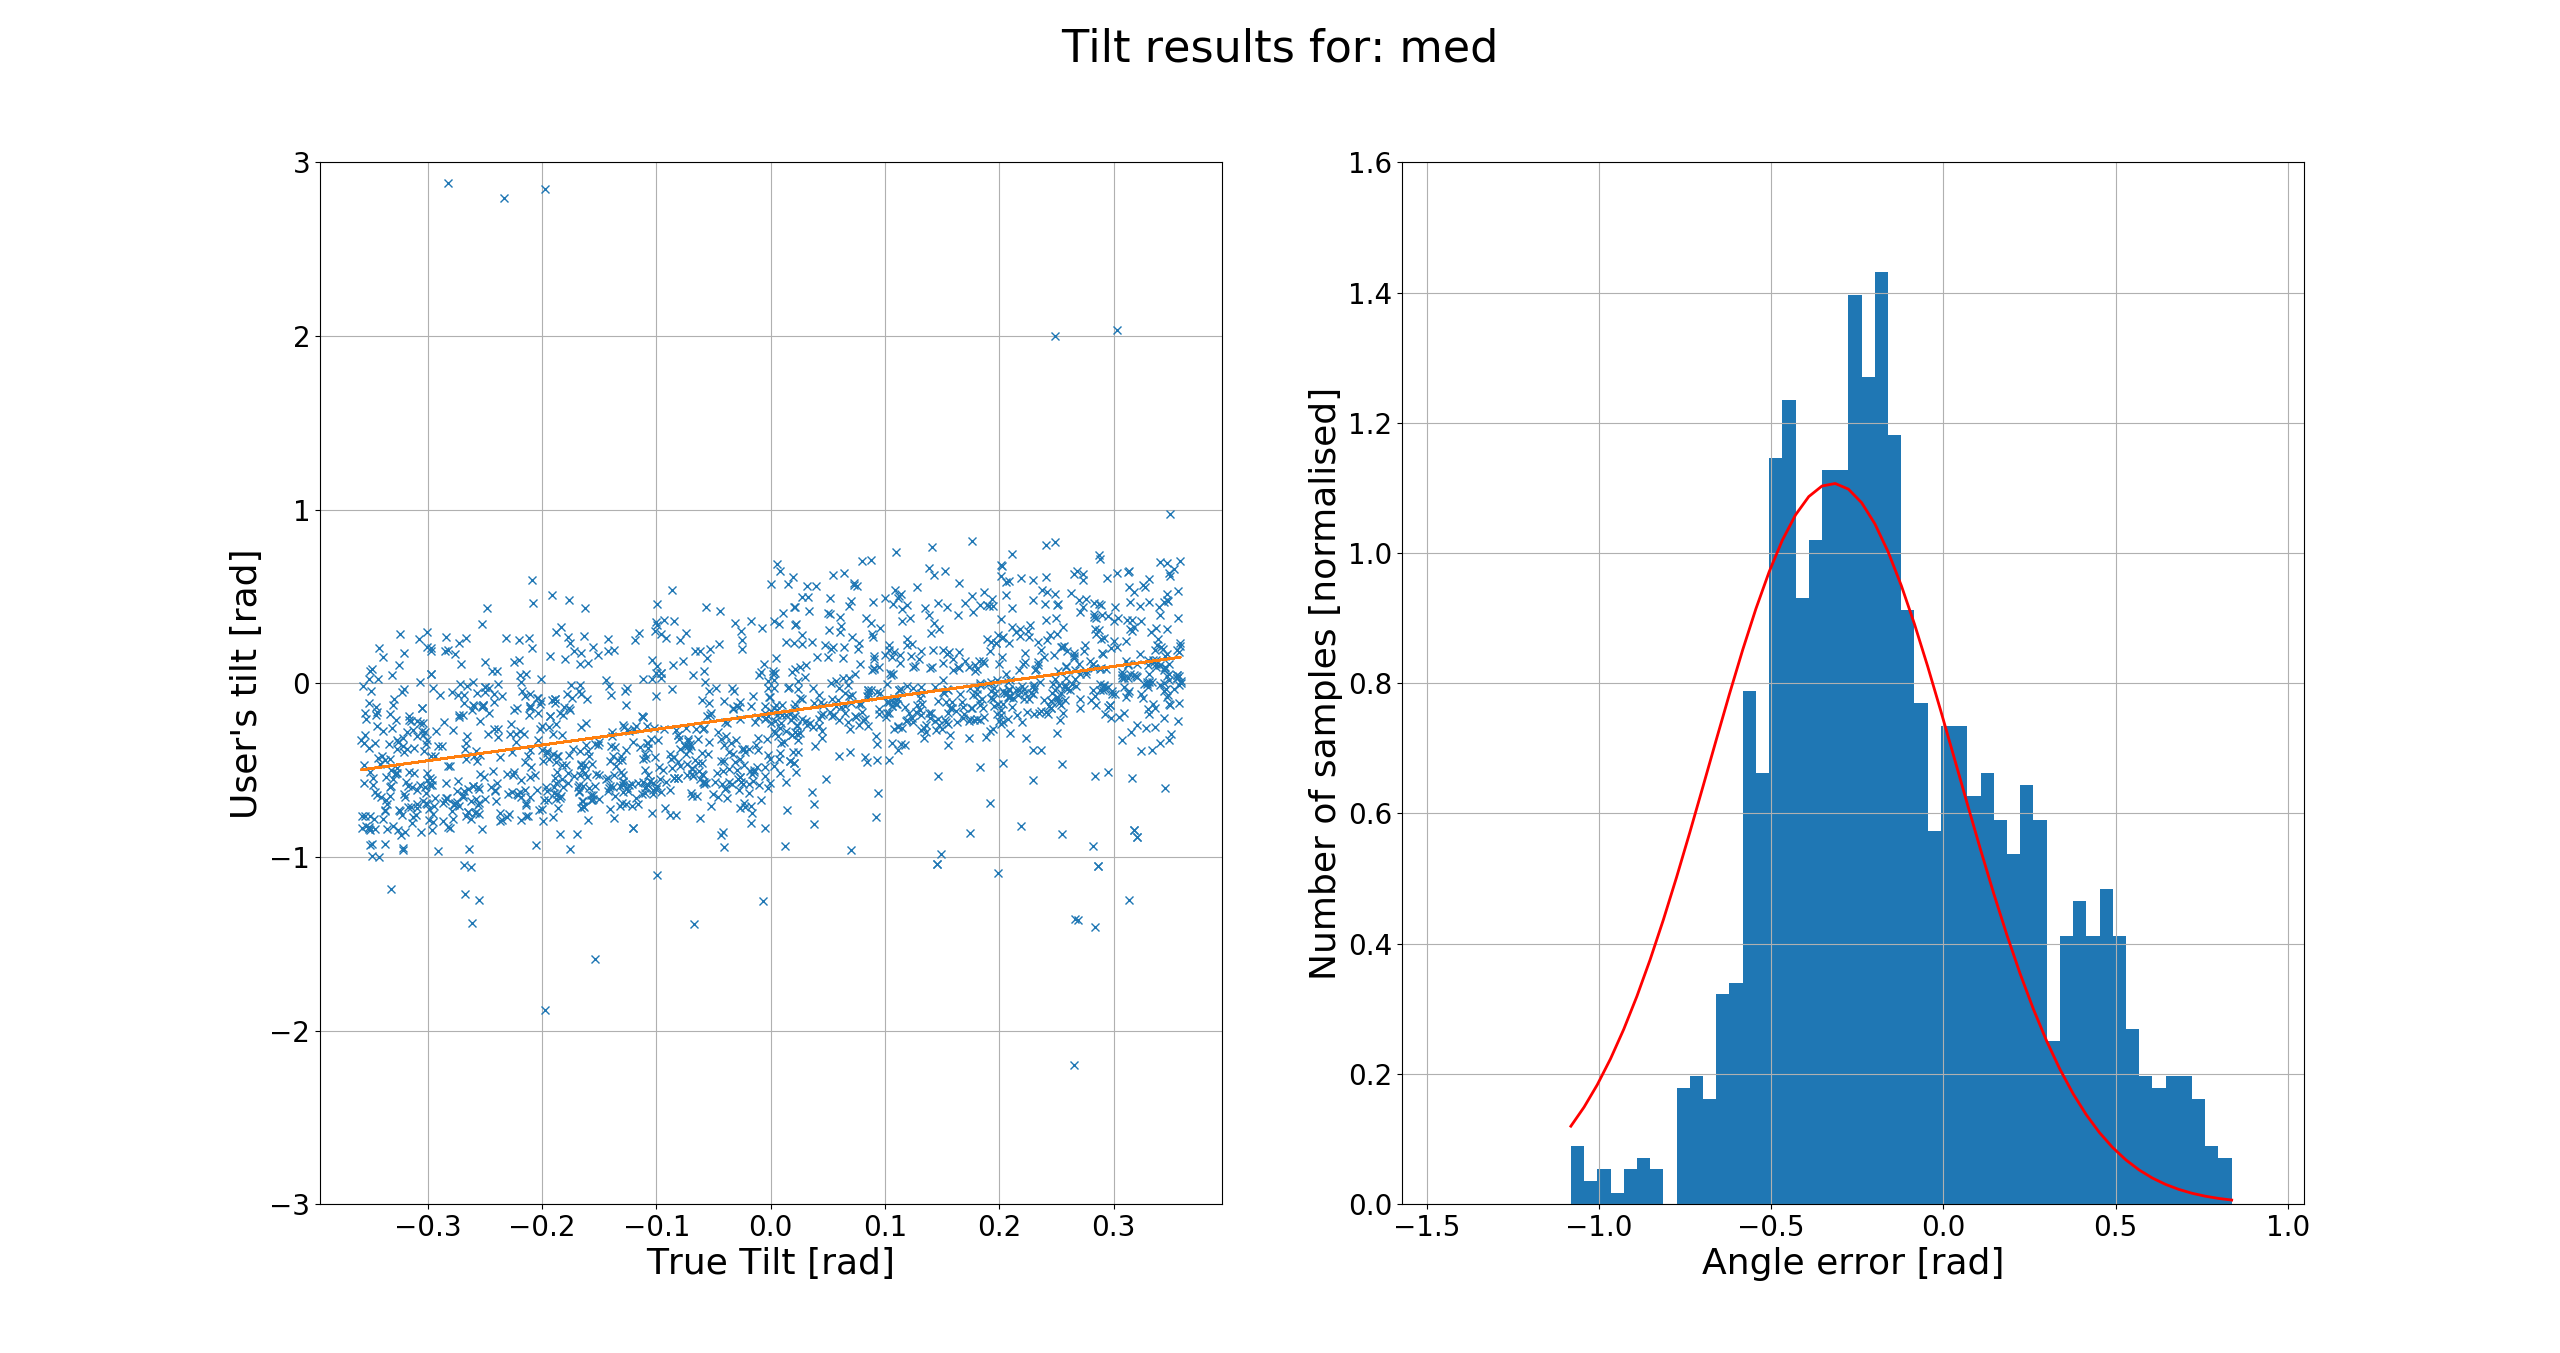
\includegraphics[width=0.5\textwidth]{figures/tilt_err_med.png}
  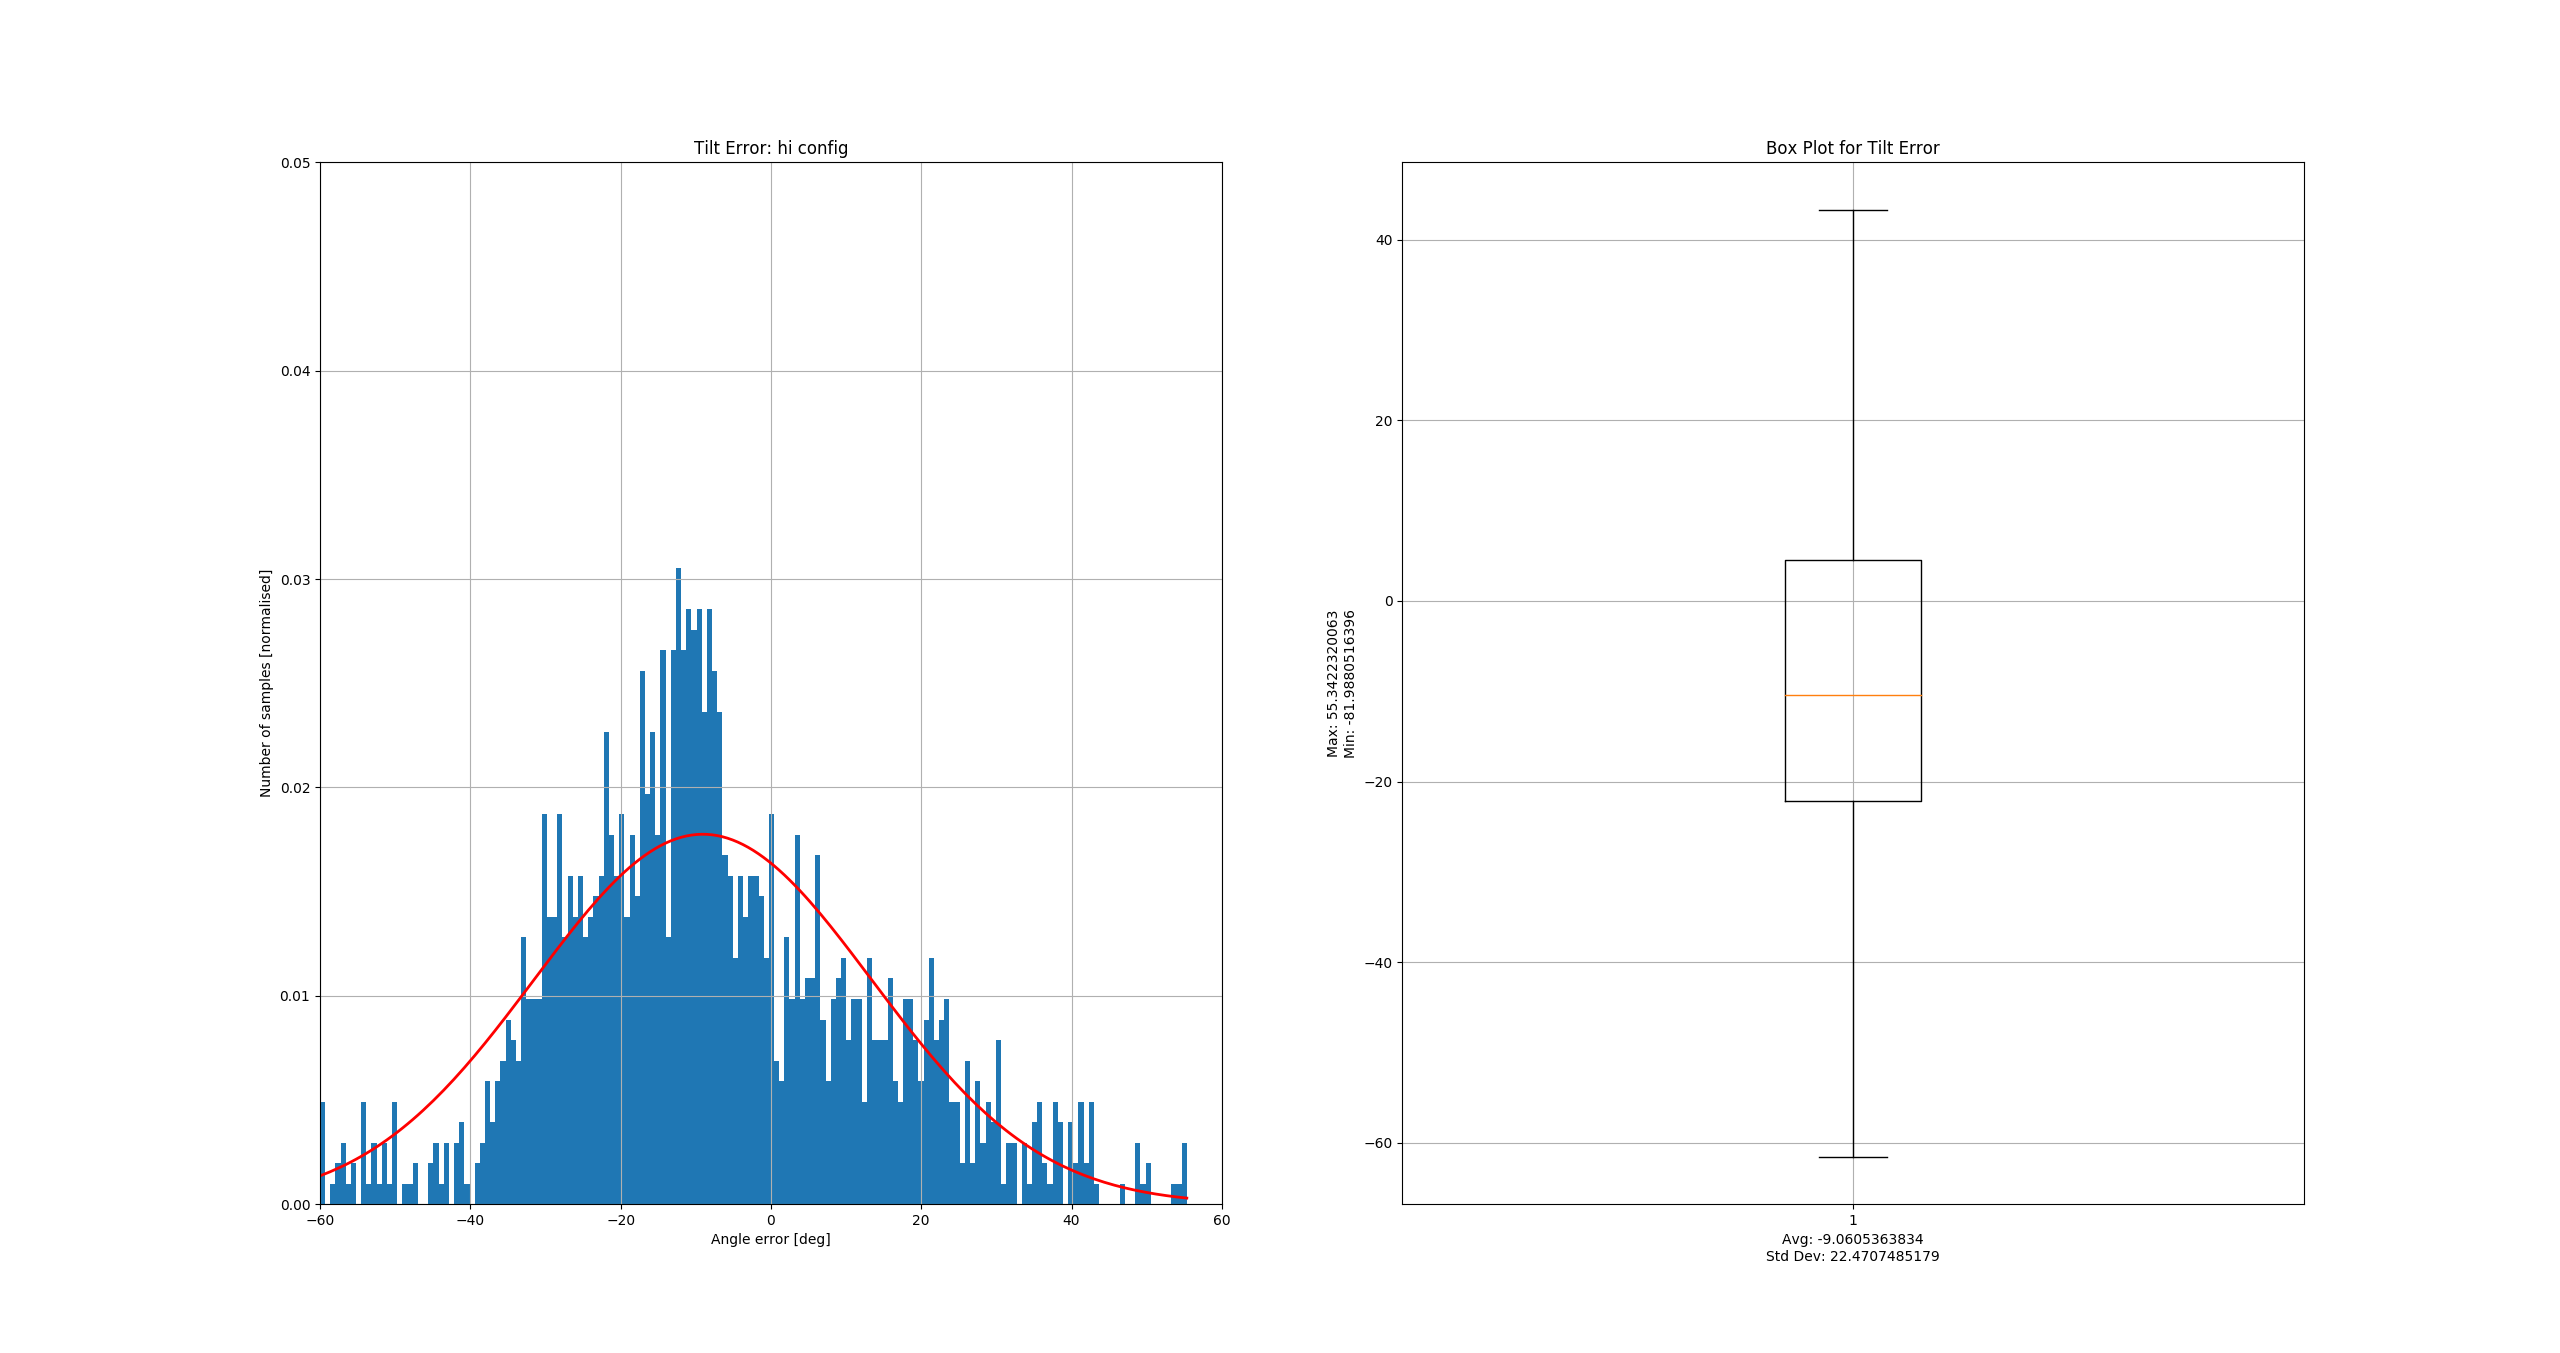
\includegraphics[width=0.5\textwidth]{figures/tilt_err_hi.png}
  \caption{The results for the target search experiment in the tilt dimension. Each plot contains the results for the \emph{lo}, \emph{med} and \emph{hi} pitch gain gradients respectively. The plot on the left is a scatter plot correlation graph between the subjects' guesses and the targets' true positions and the plots on the right are histograms for the error in these guesses. }
  \label{fig:tilt-err}
\end{figure}

\begin{figure}
  \centering
  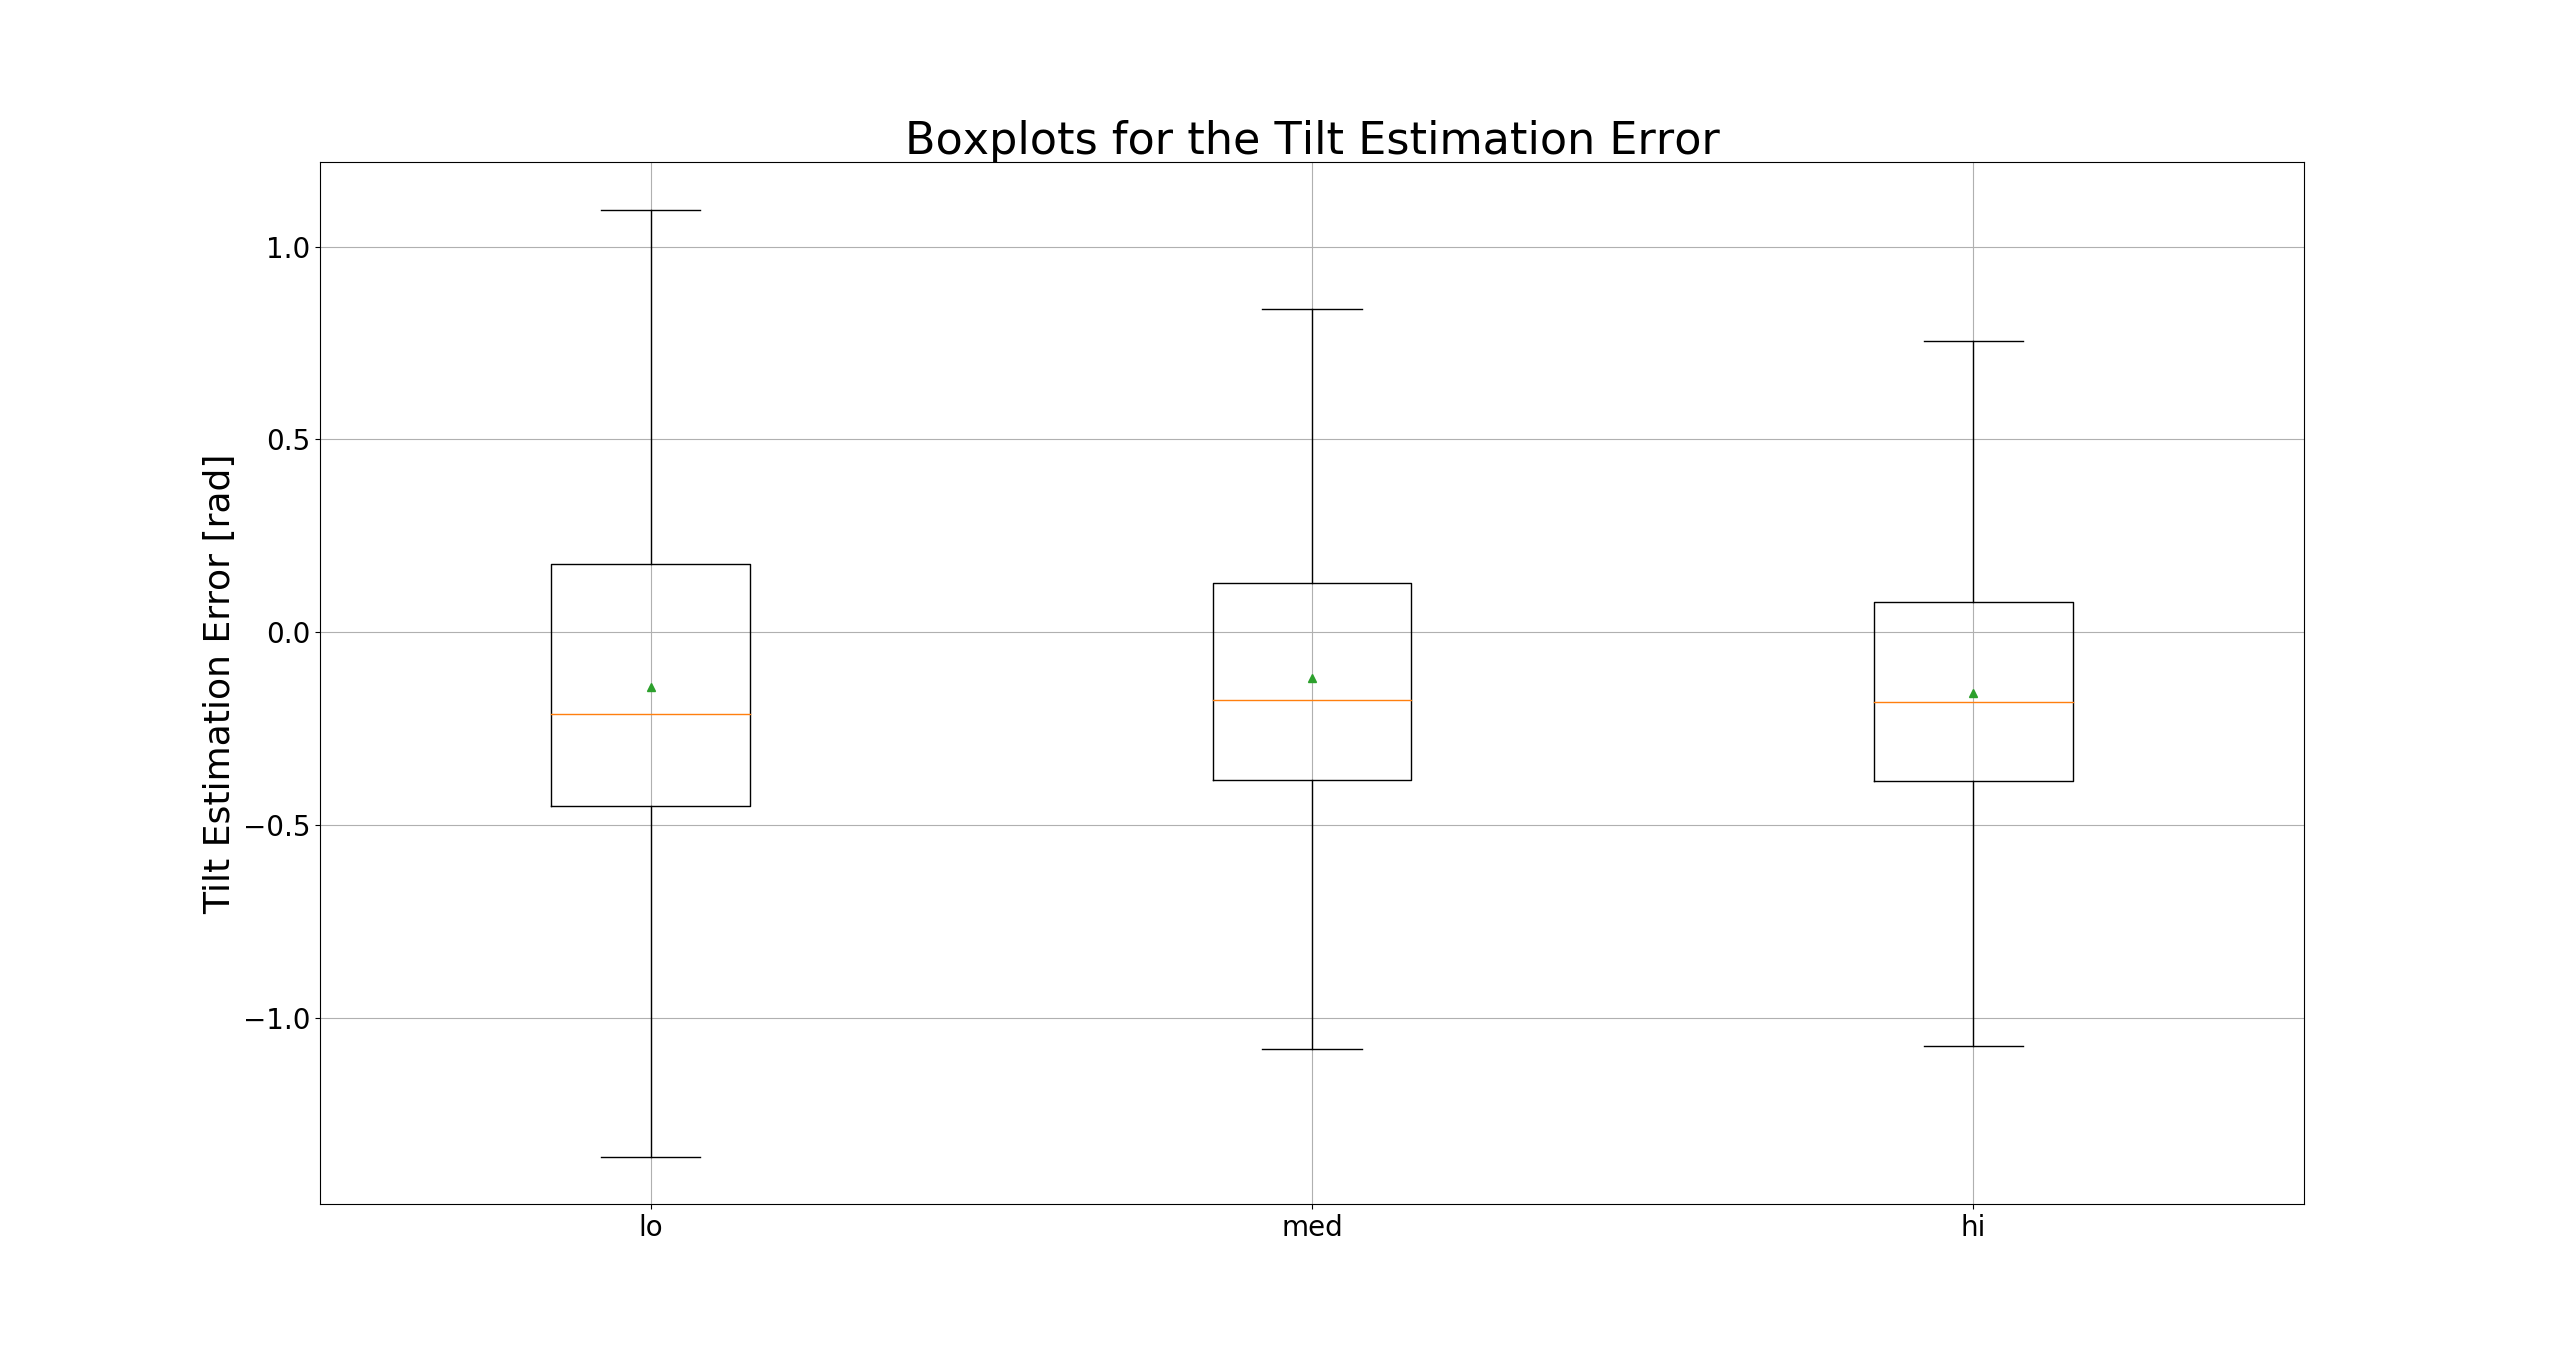
\includegraphics[width=0.5\textwidth]{figures/tilt_err_boxplot.png}
  \caption{A set of box-plots to summarise the results in the angular error data from the tilt dimension. There is a plot for each of the \emph{lo}, \emph{med} and \emph{hi} configurations. }
  \label{fig:tilt-boxplots}
\end{figure}

\begin{table}
  \centering
  \caption{A summary of the tilt results for the target search experiment. The results include the absolute average, average and standard deviations given in radians, as well as the Pearson and Spearman correlation R-scores.}
  \label{tab:tilt-results}
  \begin{tabular}{|l|l|l|l|l|l|}
    \hline
    & $\mu_{abs}$ & $\mu$ & $\sigma$ & $R_{P}$ & $R_{S}$ \\\hline\hline
    \emph{lo}  & 0.40 & -0.14 & 0.46 & 0.34 & 0.40 \\\hline
    \emph{med} & 0.32 & -0.12 & 0.36 & 0.44 & 0.52 \\\hline
    \emph{hi}  & 0.34 & -0.16 & 0.39 & 0.48 & 0.55 \\\hline
  \end{tabular}
\end{table}

We can see from the plots that there is a relatively strong linear correlation between the user's guesses and the actual locations of the targets, indicating that the varying pitch is working as expected and the subjects in general are interpreting the cues correctly. This is supported by the Pearson correlation coefficient of the datasets that equate to 0.34, 0.44 and 0.48 for the \emph{lo}, \emph{med} and \emph{hi} configurations respectively, each with a statistical significance lower than 5\%, indicating that it is reasonable to trust the correlation scores. The Spearman correlation scores are 0.40, 0.52, 0.55 for each respective dataset with a significance level still below 5\%. 

The average errors of the datasets are closer to one another, with the \emph{lo} gradient giving the largest absolute error at \SI{0.46}{\radian} and the \emph{med} and \emph{hi} a similar absolute error of \SI{0.36}{\radian} and \SI{0.39}{\radian} respectively. This is in line with the correlation scores with the \emph{lo} gradient giving a significantly worse result than the \emph{med} and \emph{hi} gradients and the \emph{hi} gradient giving the best results overall with its high correlation score and relatively low absolute angular errors and standard deviation. 

It can also be seen that the data is not normally spread and displays a significant skewing to the negative side indicating a potential bias amongst the experiment subject-base that must be taken into account. This non-normality makes analysing the mean data with the conventional t-test and analysis of variance unreliable (ANOVA). We therefore use the non-parametric versions of the ANOVA test, i.e. the Kruskal-Wallis test~\cite{kruskal1952use} and Mood's median test~\cite{mood1950introduction}, to show the statistical difference between the datasets. The results show that the $p$-values fall outside of the critical 10\% threshold, meaning that the results from the three datasets are statistically different from one another, but the $p$-value for Kruskal-Wallis test falls very closely on the boundary. The values are shown in Table~\ref{tab:tilt-stats}.

\begin{table}
  \centering
  \caption{The results of the standard ANOVA test, as well as the Kruskal-Wallis and Mood's non-parametric versions of the ANOVA test.}
  \label{tab:tilt-stats}
  \begin{tabular}{|l|l|l|}
    \hline
    $p_{ANOVA}$ & $p_{KW}$ & $p_{M}$ \\\hline
    2.91\% & 9.06\% & 5.31\% \\\hline
  \end{tabular}
\end{table}

At this stage it is unclear what causes this bias, but it is suspected that the ground introduced a position constraint within the subjects' minds, where the target could not appear below the ground, but can potentially appear well above the subjects' head, giving variable upper an lower limits that are dependant on the subjects' height and individual perception. We might have to consider using a non-linear increase in pitch as a function of tilt angle instead of the linear one we used for these experiments to remedy this bias. The skewness of the data makes it impossible to use 

These results highlight a clear and significant difference between the three different pitch gain gradients, with the steep-gradient gain in pitch as a function of target tilt angle producing the results closest to the true tilt. Moreover, it shows that a tone with varying pitch can be used to convey the tilt angle of a virtual target to a human user to a degree of accuracy similar to those previously established in literature~\cite{bujacz2011sonification, katz2011spatial, zotkin2004rendering} using spatial sound, either with an HRTF or mobile speakers, and a head-mounted orientation tracker.

\subsubsection{Panning Results}

The results from the target search experiment in the pan dimension are given in Figure~\ref{fig:pan-err}, where a scatter plot of the subjects' guesses vs. the target's actual location are given along with a histogram of the error data between the subjects' guesses and the targets' actual positions. A set of box-plots of the angular errors are also given in Figure~\ref{fig:pan-boxplots}. A plot for each of the \emph{lo}, \emph{med} and \emph{hi} configurations are given. The results are summarised in Table~\ref{tab:pan-results}.

\begin{figure}
  \centering
  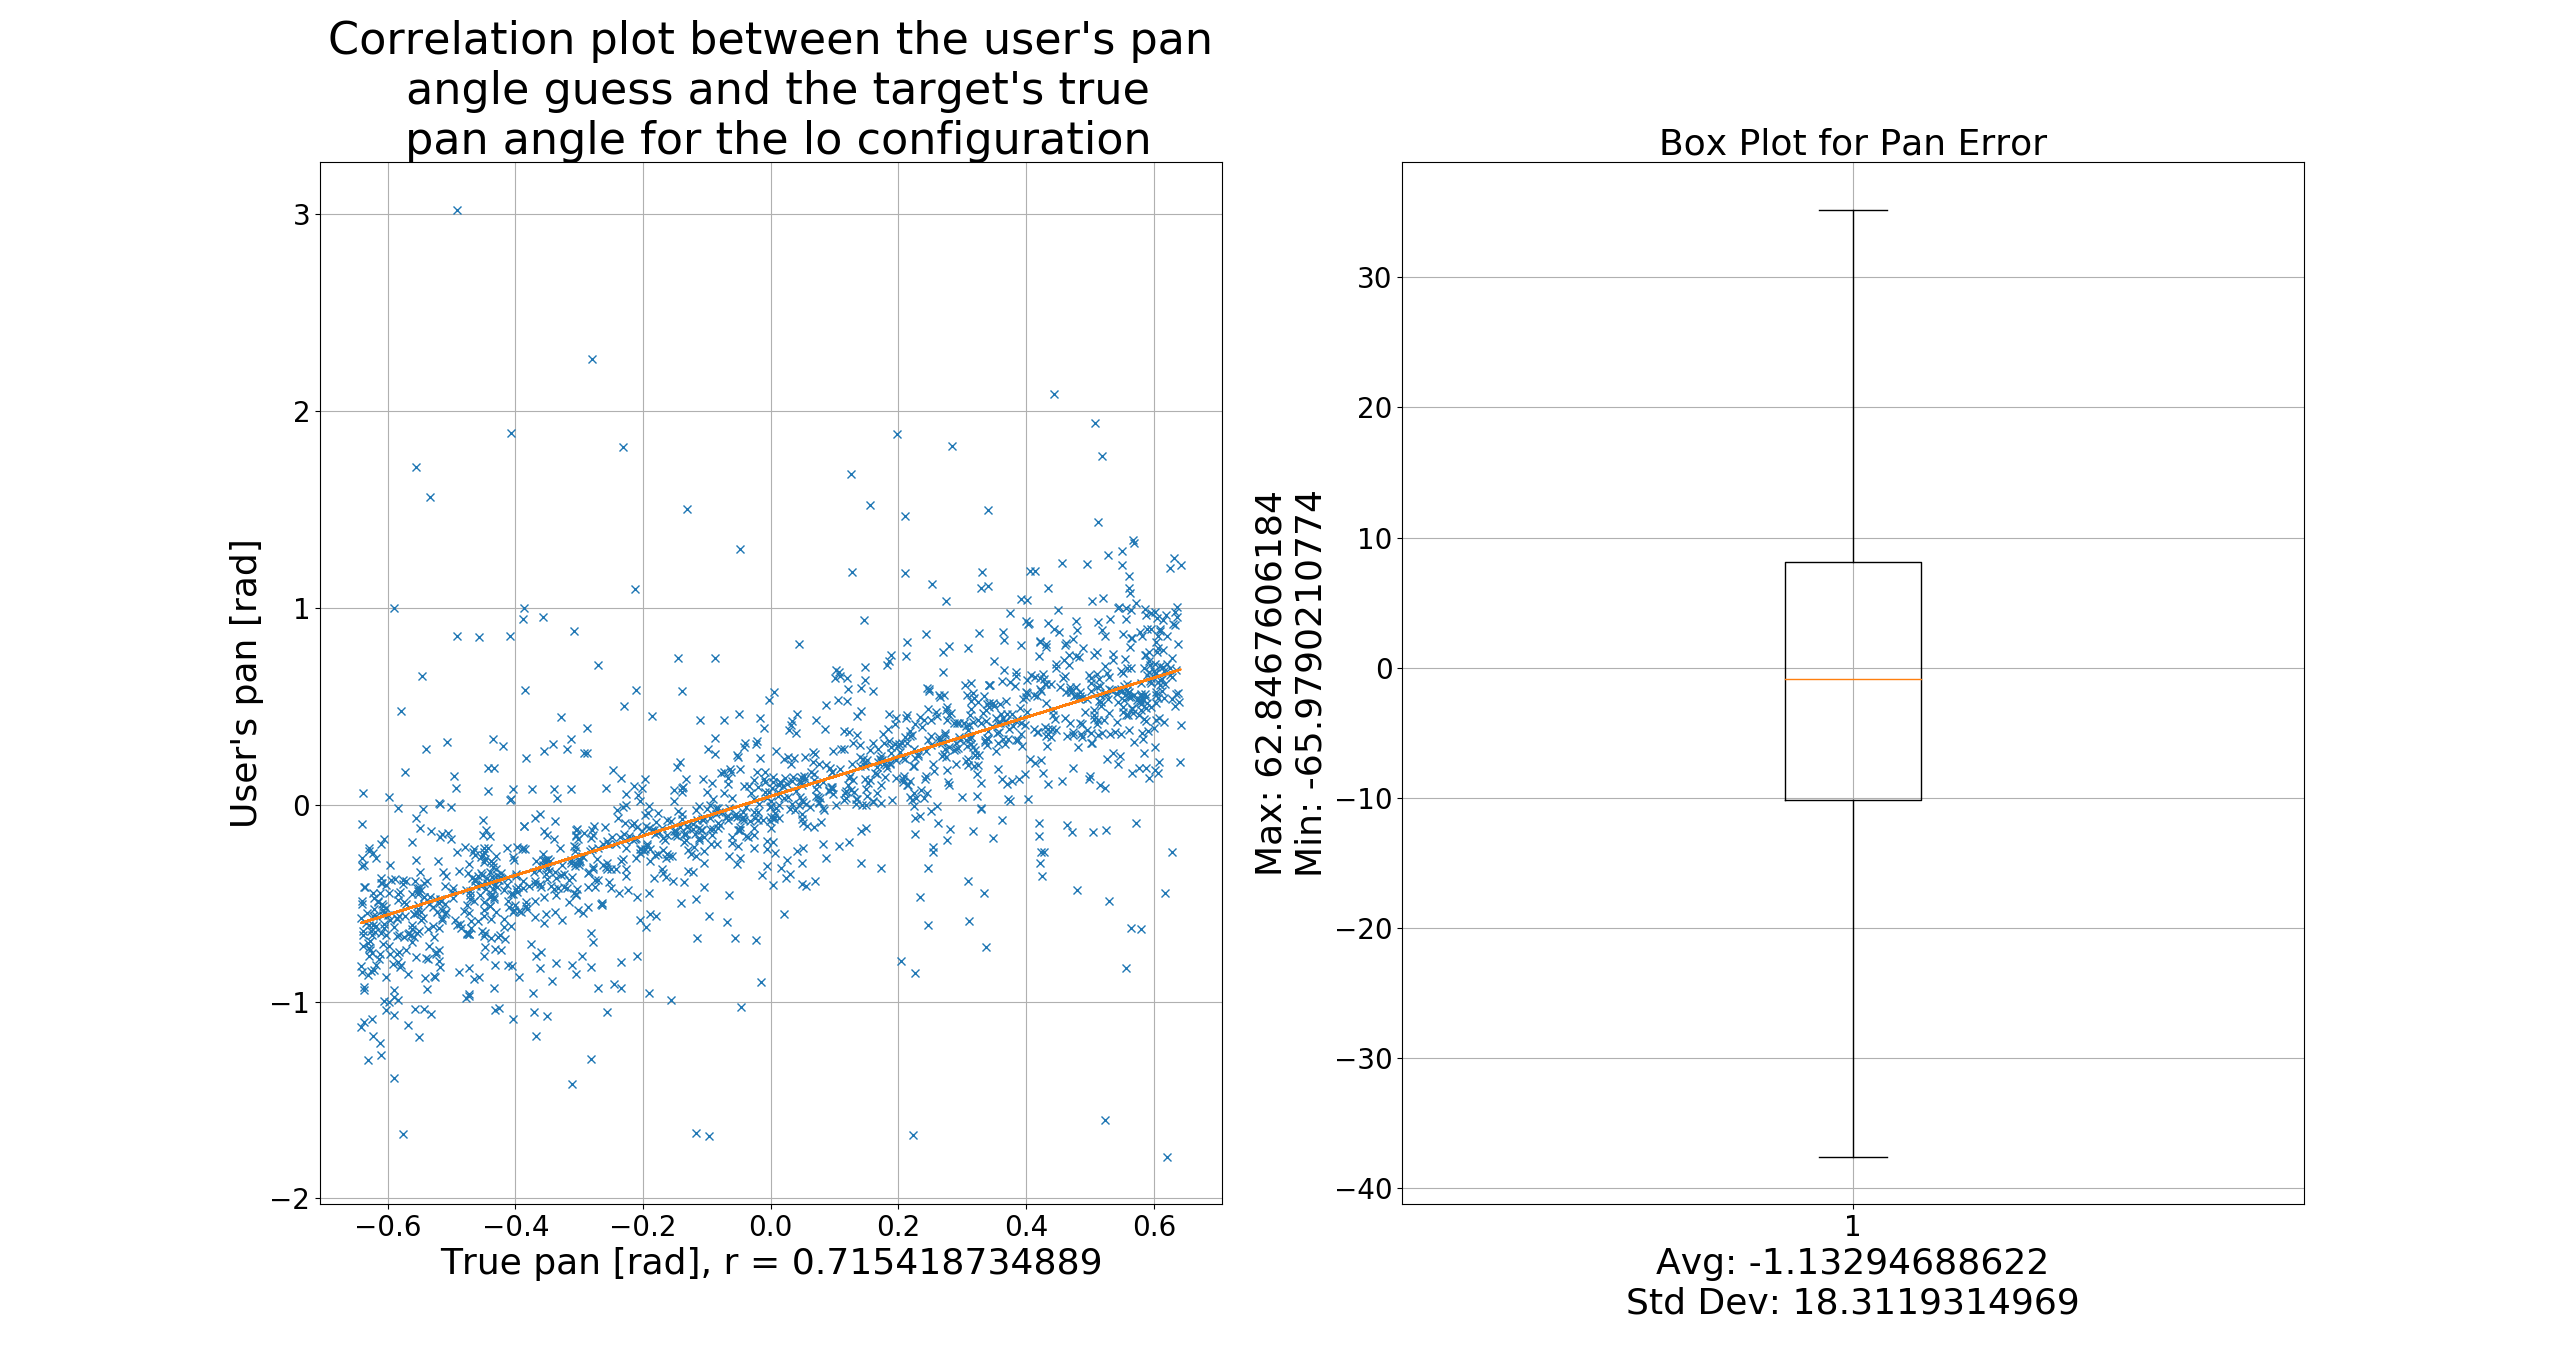
\includegraphics[width=0.5\textwidth]{figures/pan_err_lo.png}
  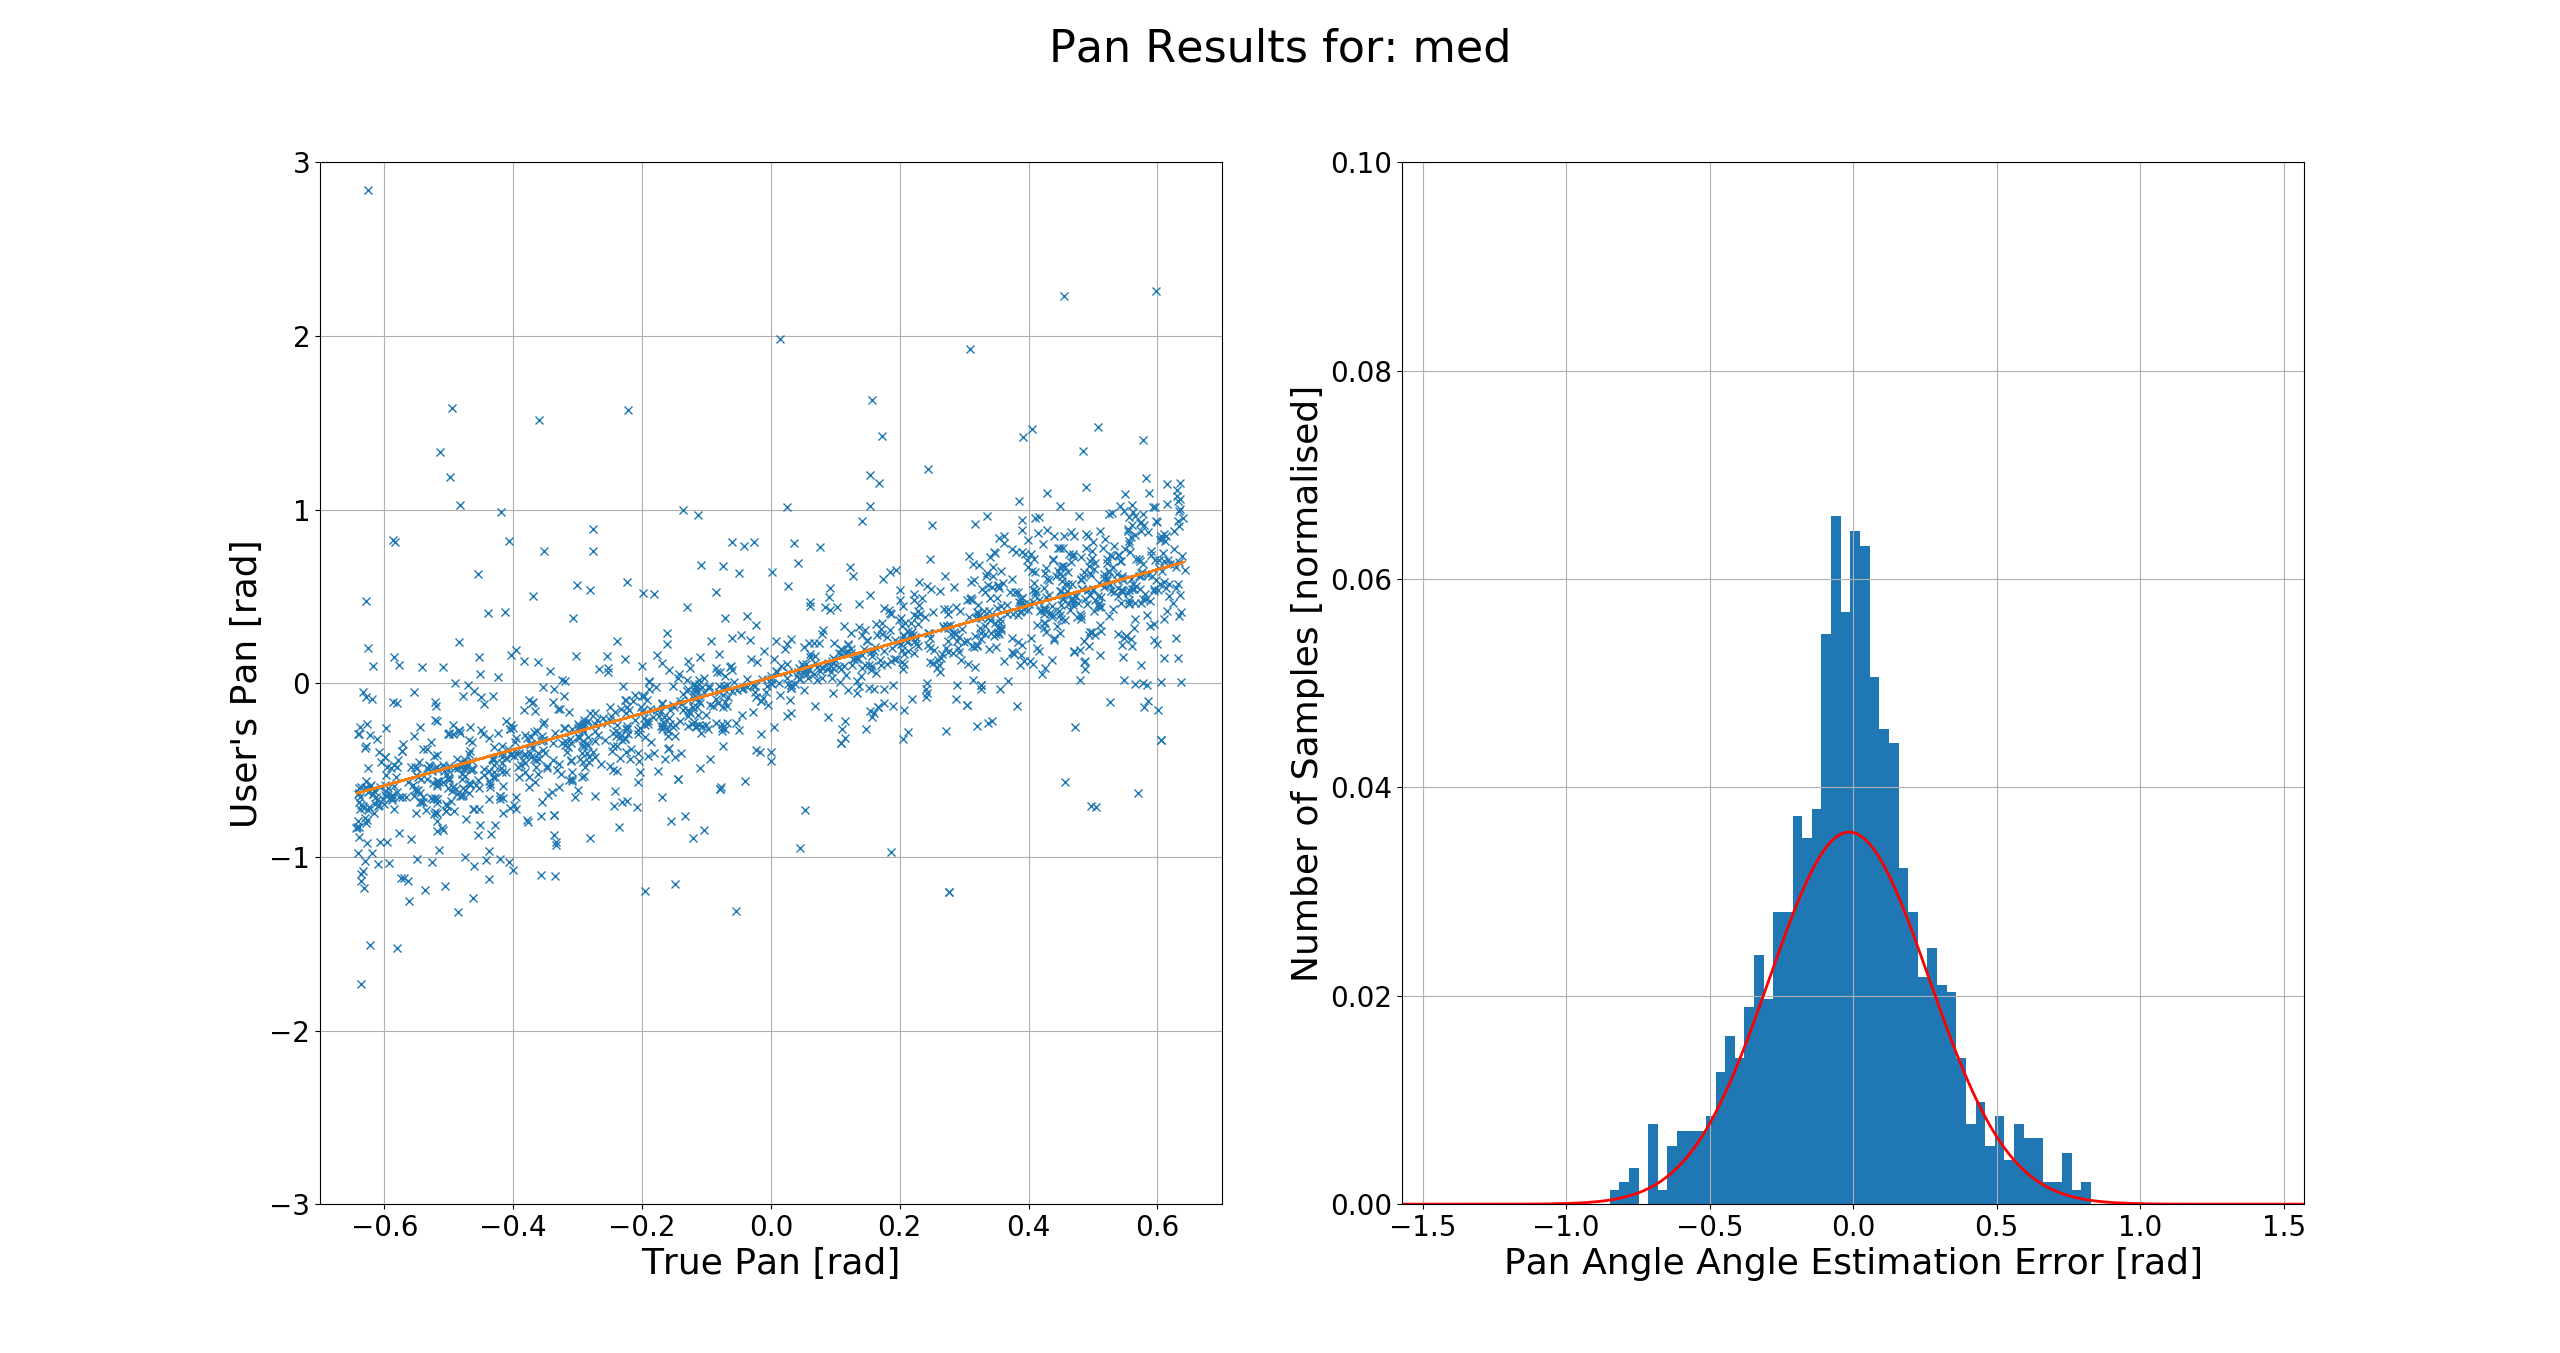
\includegraphics[width=0.5\textwidth]{figures/pan_err_med.png}
  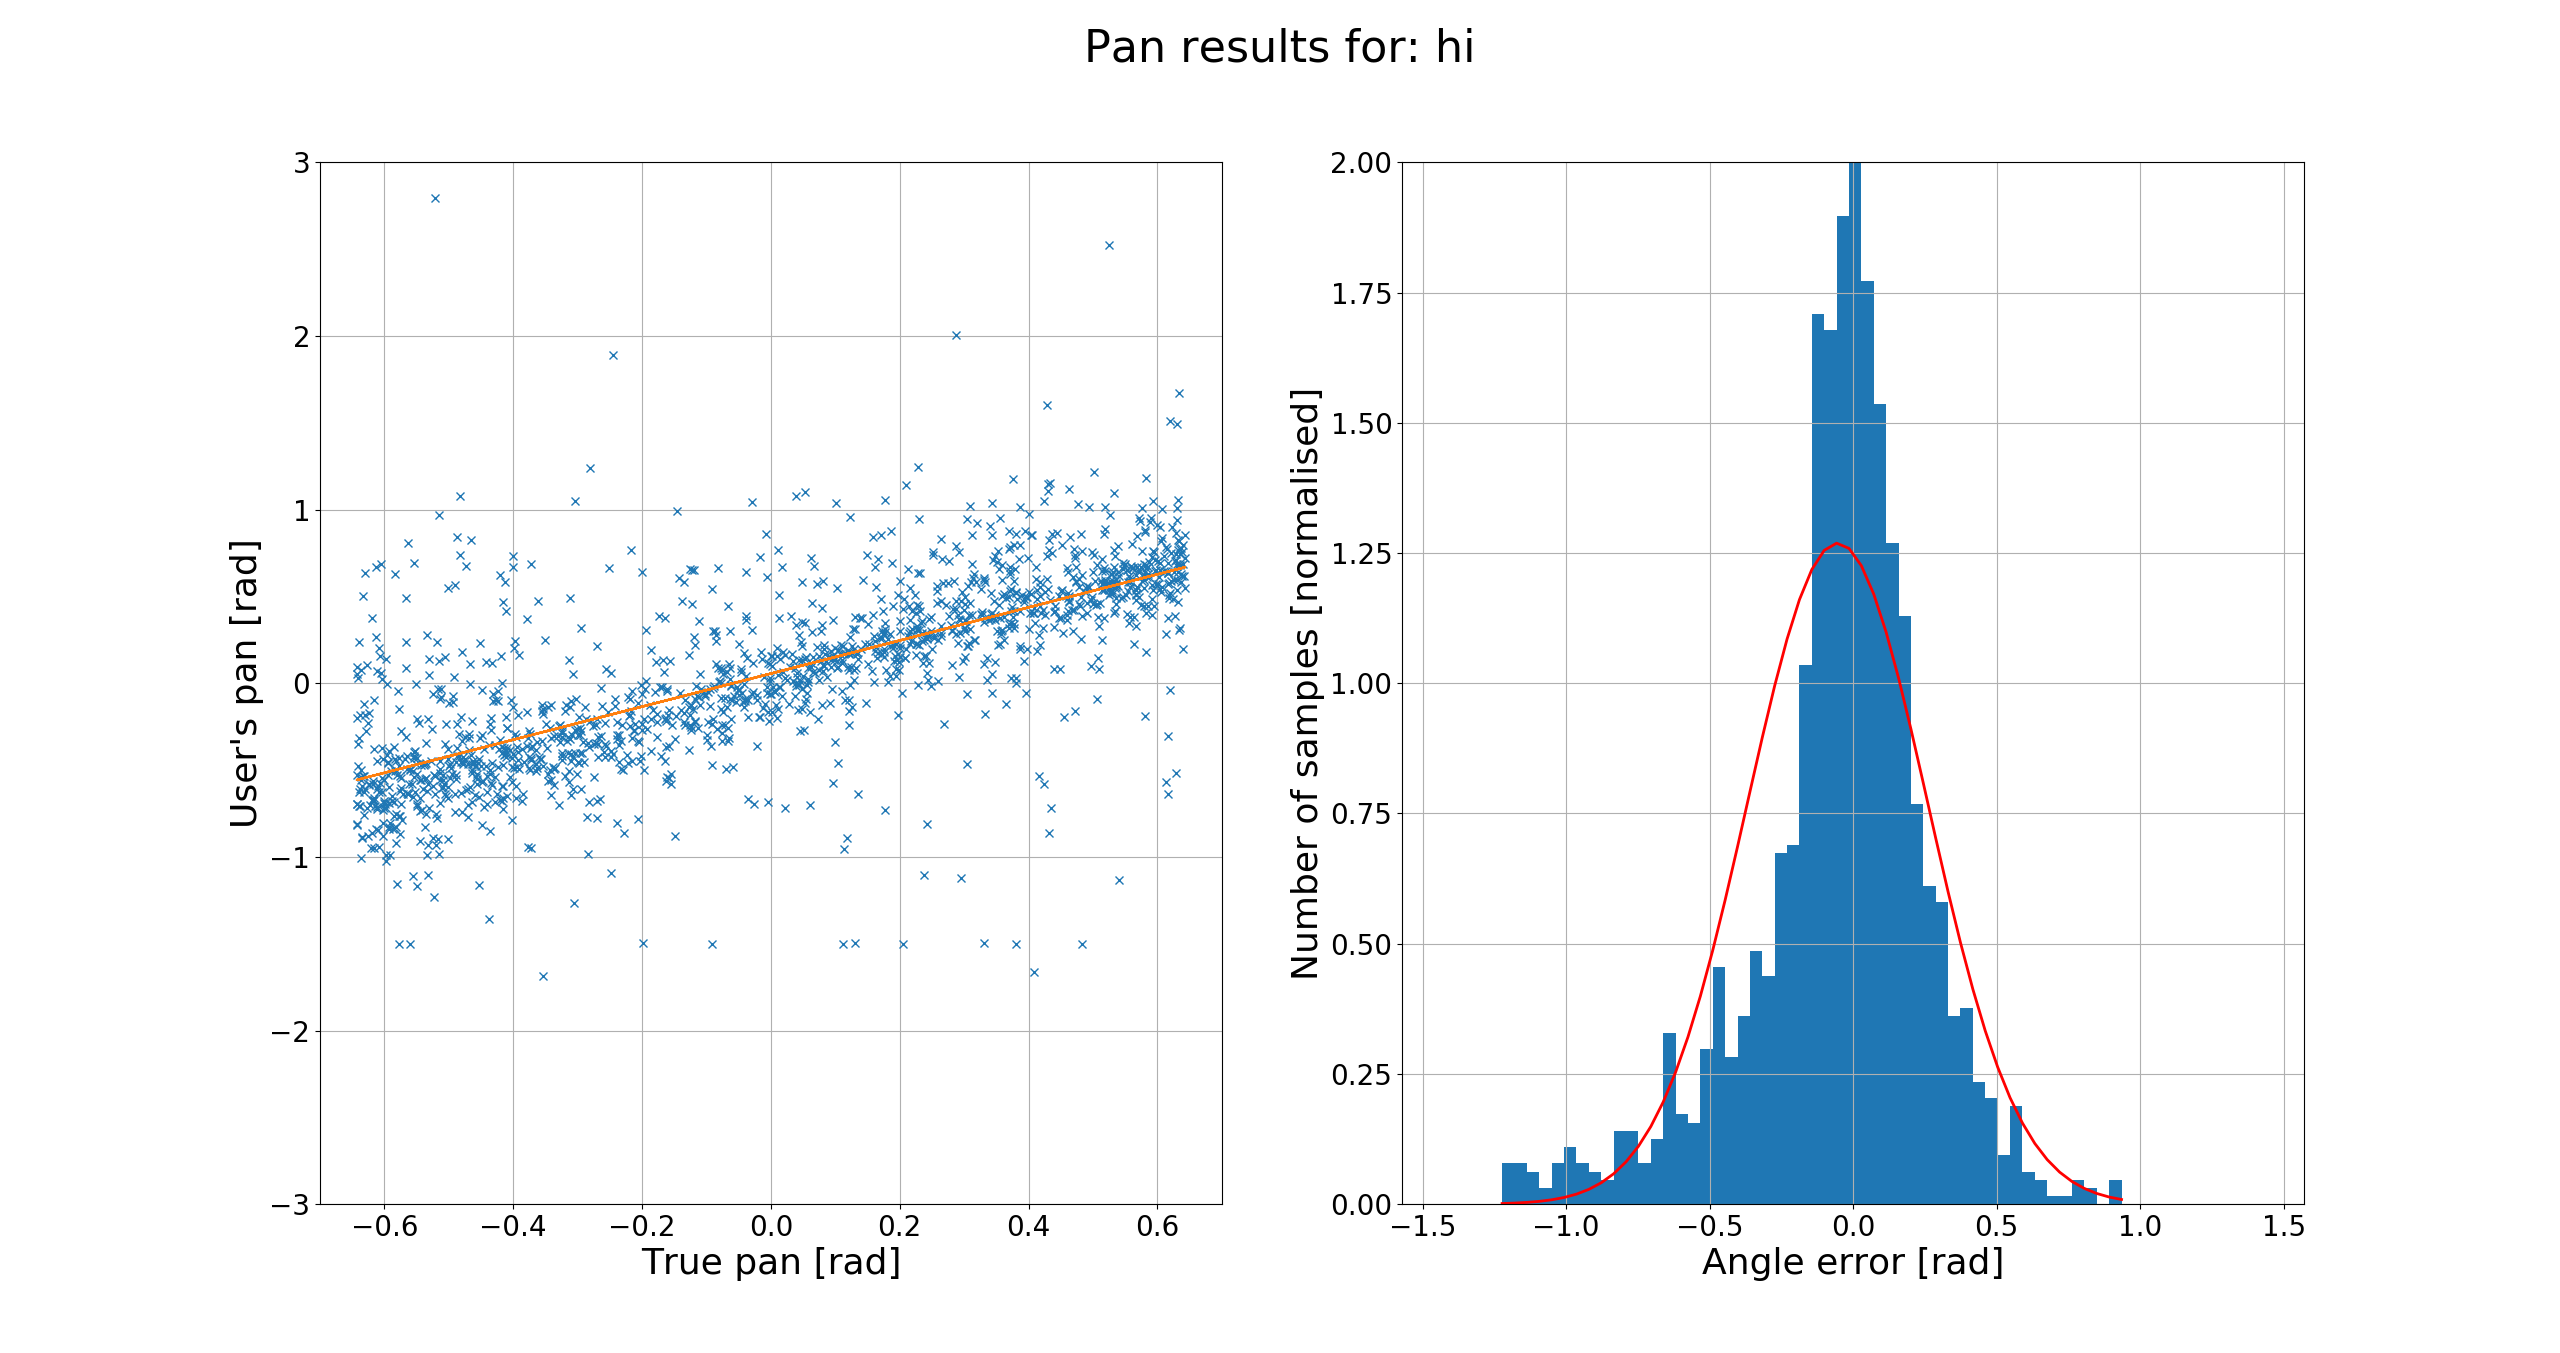
\includegraphics[width=0.5\textwidth]{figures/pan_err_hi.png}
  \caption{The results for the target search experiment in the pan dimension. Each plot contains the results for the \emph{lo}, \emph{med} and \emph{hi} pitch gain gradients respectively. The plot on the left is a scatter plot correlation graph between the subjects' guesses and the targets' true positions and the plots on the right are histograms for the error in these guesses. }
  \label{fig:pan-err}
\end{figure}

\begin{figure}
  \centering
  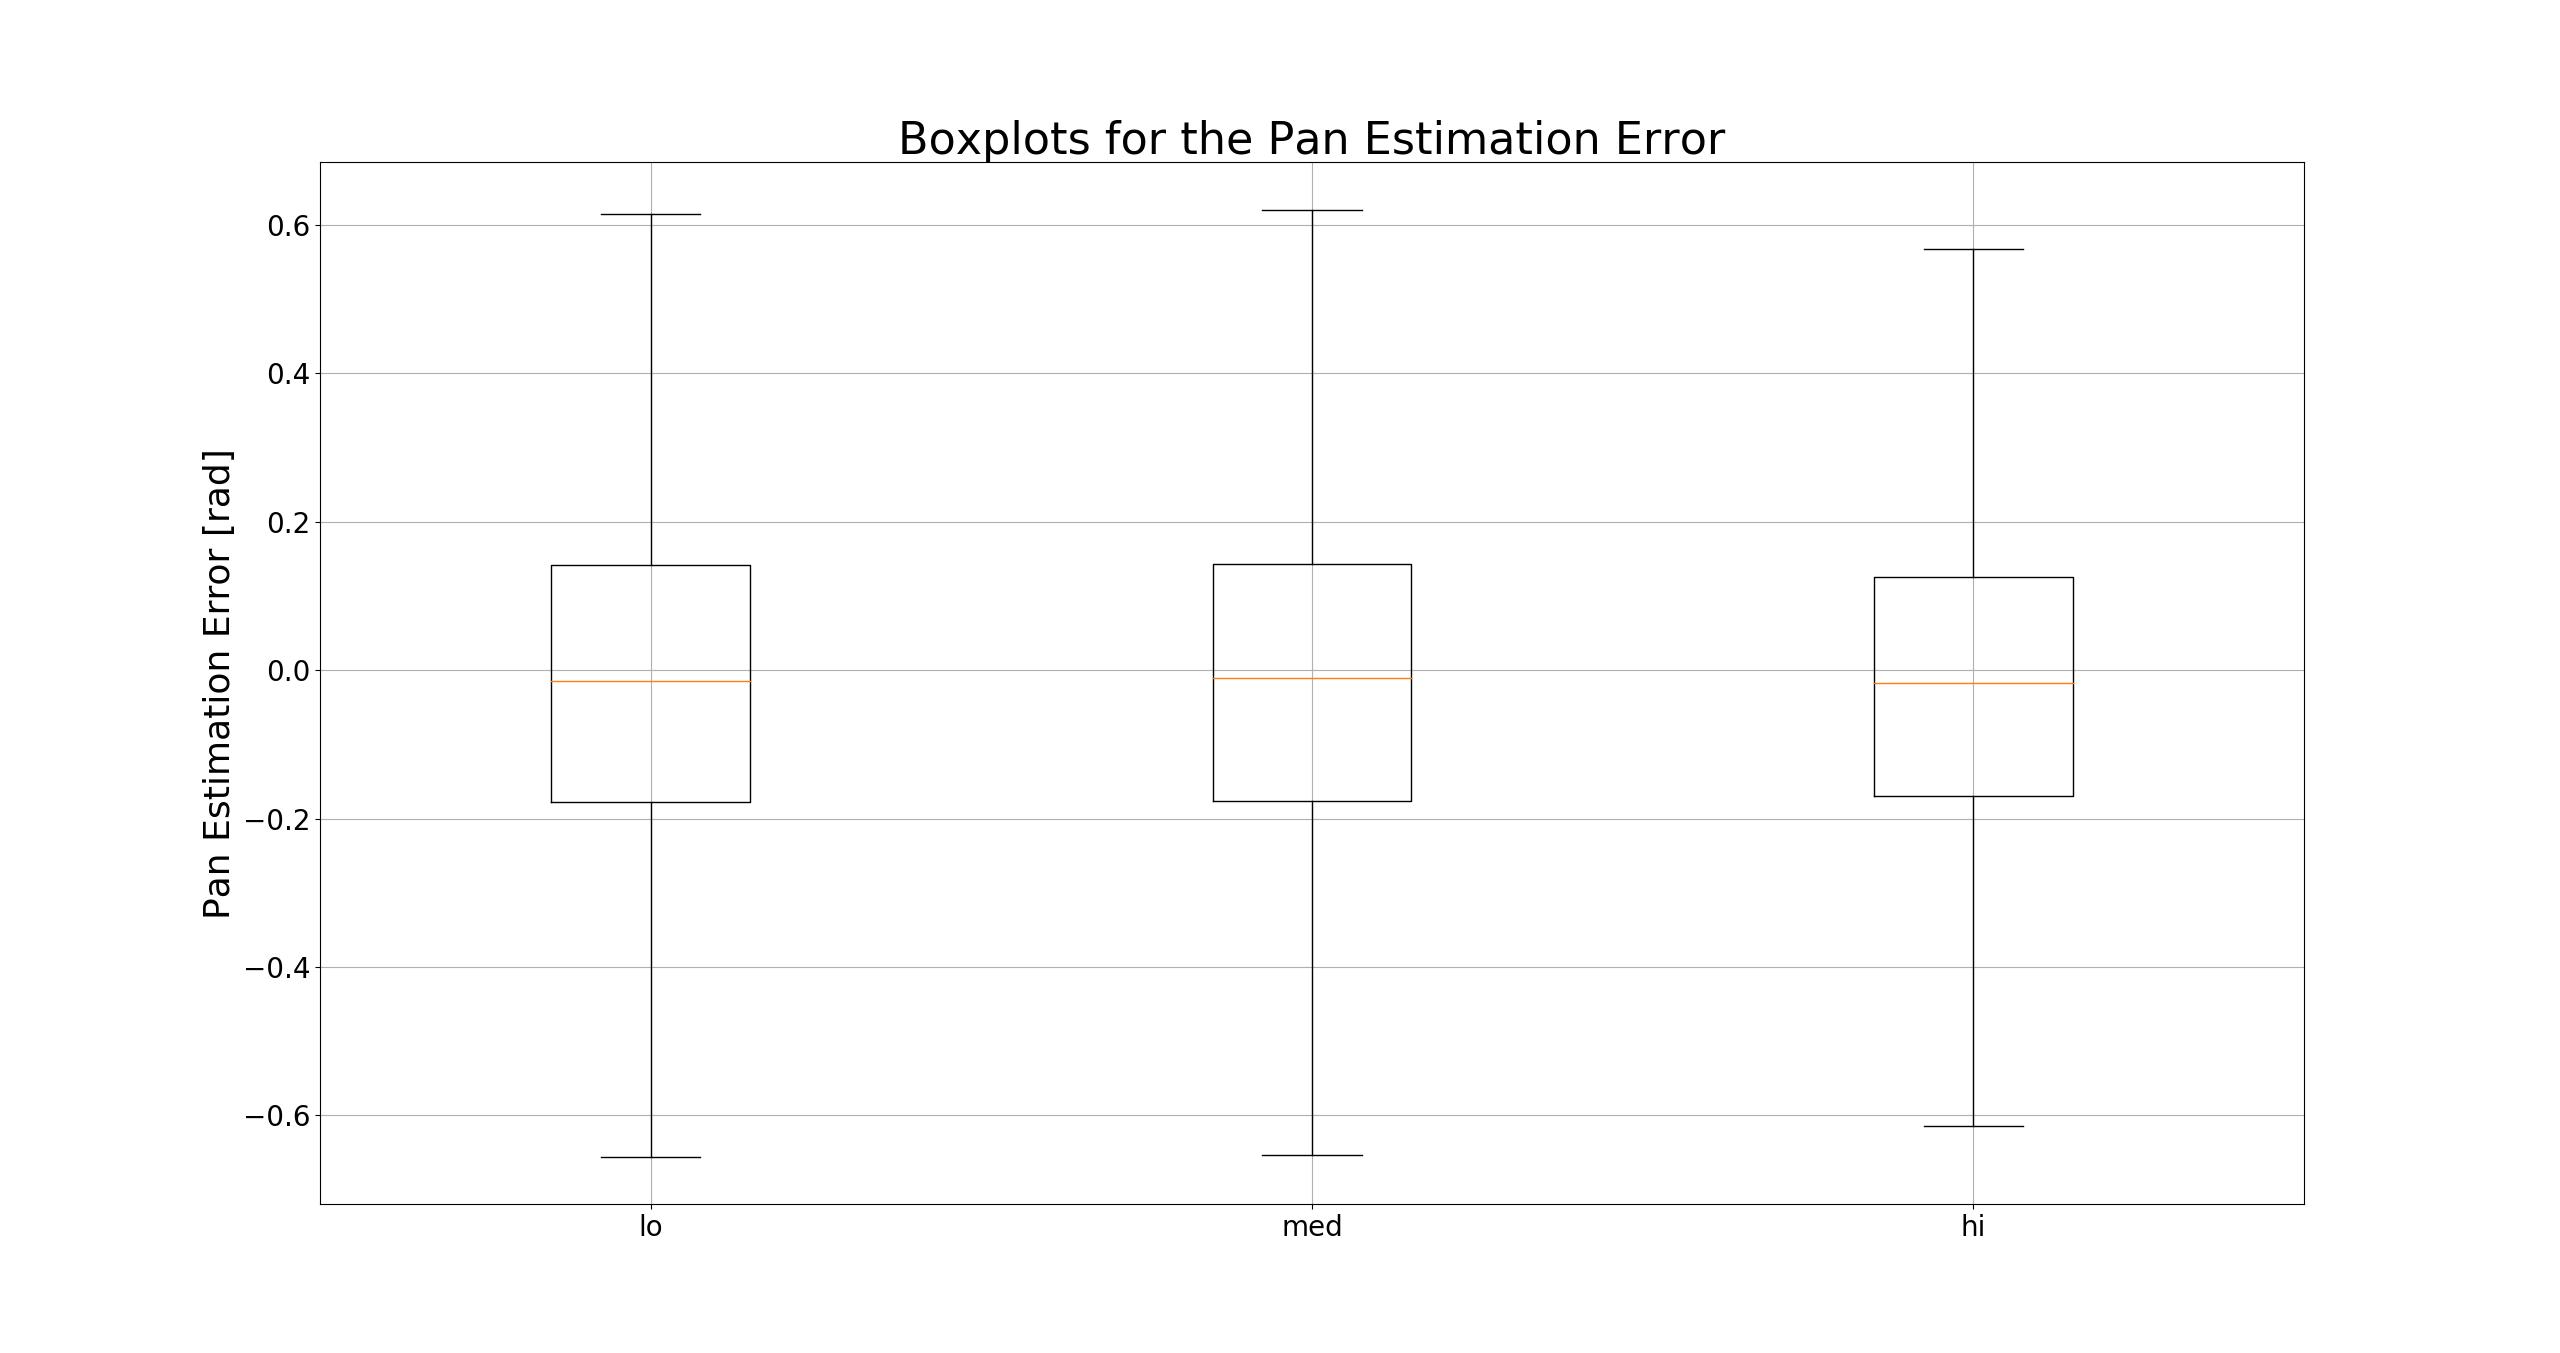
\includegraphics[width=0.5\textwidth]{figures/pan_err_boxplot.png}
  \caption{A plot showing a histogram of the pan errors, along with the corresponding box plots. }
  \label{fig:pan-err-boxplots}
\end{figure}

\begin{table}
  \centering
  \caption{A summary of the pan results for the target search experiment. The results include the absolute average, average and standard deviations given in radians, as well as the Pearson and Spearman correlation R-scores.}
  \label{tab:pan-results}
  \begin{tabular}{|l|l|l|l|l|l|}
    \hline
    & $\mu_{abs}$ & $\mu$ & $\sigma$ & $R_{P}$ & $R_{S}$ \\\hline\hline
    \emph{lo}  & 0.23 & -0.02 & 0.32 & 0.72 & 0.78 \\\hline
    \emph{med} & 0.21 & -0.01 & 0.28 & 0.76 & 0.80 \\\hline
    \emph{hi}  & 0.22 & -0.05 & 0.31 & 0.71 & 0.75 \\\hline
  \end{tabular}
\end{table}

The scatter plots display evidence of a very strong linear correlation between the subjects' guesses and the targets' true pan angles. This is confirmed by both the Pearson and Spearman correlation scores of above 0.7 for all three datasets, with the \emph{med} configuration displaying the best result at 0.75 for the Pearson score and 0.8 for the Pearson, with a statistical level of significance well below 5\%. 

The angular errors are roughly normally distributed around zero with comparable average errors and standard deviations, with the \emph{med} configuration producing the best results with the smallest average error and standard deviation. However, the differences are not big enough (approximately 6\% difference, ANOVA $p$-value of less than 5\%) to conclude that the pitch gradient has a clear effect on the performance. The results of the 
[CHECK WTF HIER AANGAAN]

\begin{table}
  \centering
  \caption{The results of the standard ANOVA test, as well as the Kruskal-Wallis and Mood's non-parametric versions of the ANOVA test.}
  \label{tab:tilt-stats}
  \begin{tabular}{|l|l|l|}
    \hline
    $p_{ANOVA}$ & $p_{KW}$ & $p_{M}$ \\\hline
    0.056\% & 21.5\% & 80\% \\\hline
  \end{tabular}
\end{table}

Based on previous research results, these results were somewhat expected. However, they also confirm that the target search capability of a subject in the pan dimension is fairly robust to the changing pitch we used to convey the target's tilt location which is a useful result going forward. %The smallest angular error and highest correlation was achieved when the med gain gradient for the pitch was used. However, the difference between these values here is not significant enough to conclude that the varying pitch has a significant effect on the accuracy of the target search in the pan dimension. 

\subsection{Time to Target}

We used the relation from Equation~\ref{eq:fitts-simple} and fitted a line through the distance-time data we gathered. The resulting plots are given in Figure~\ref{fig:fitts}.% to~\ref{fig:fitts-hi}. 

\begin{figure}
  \centering
  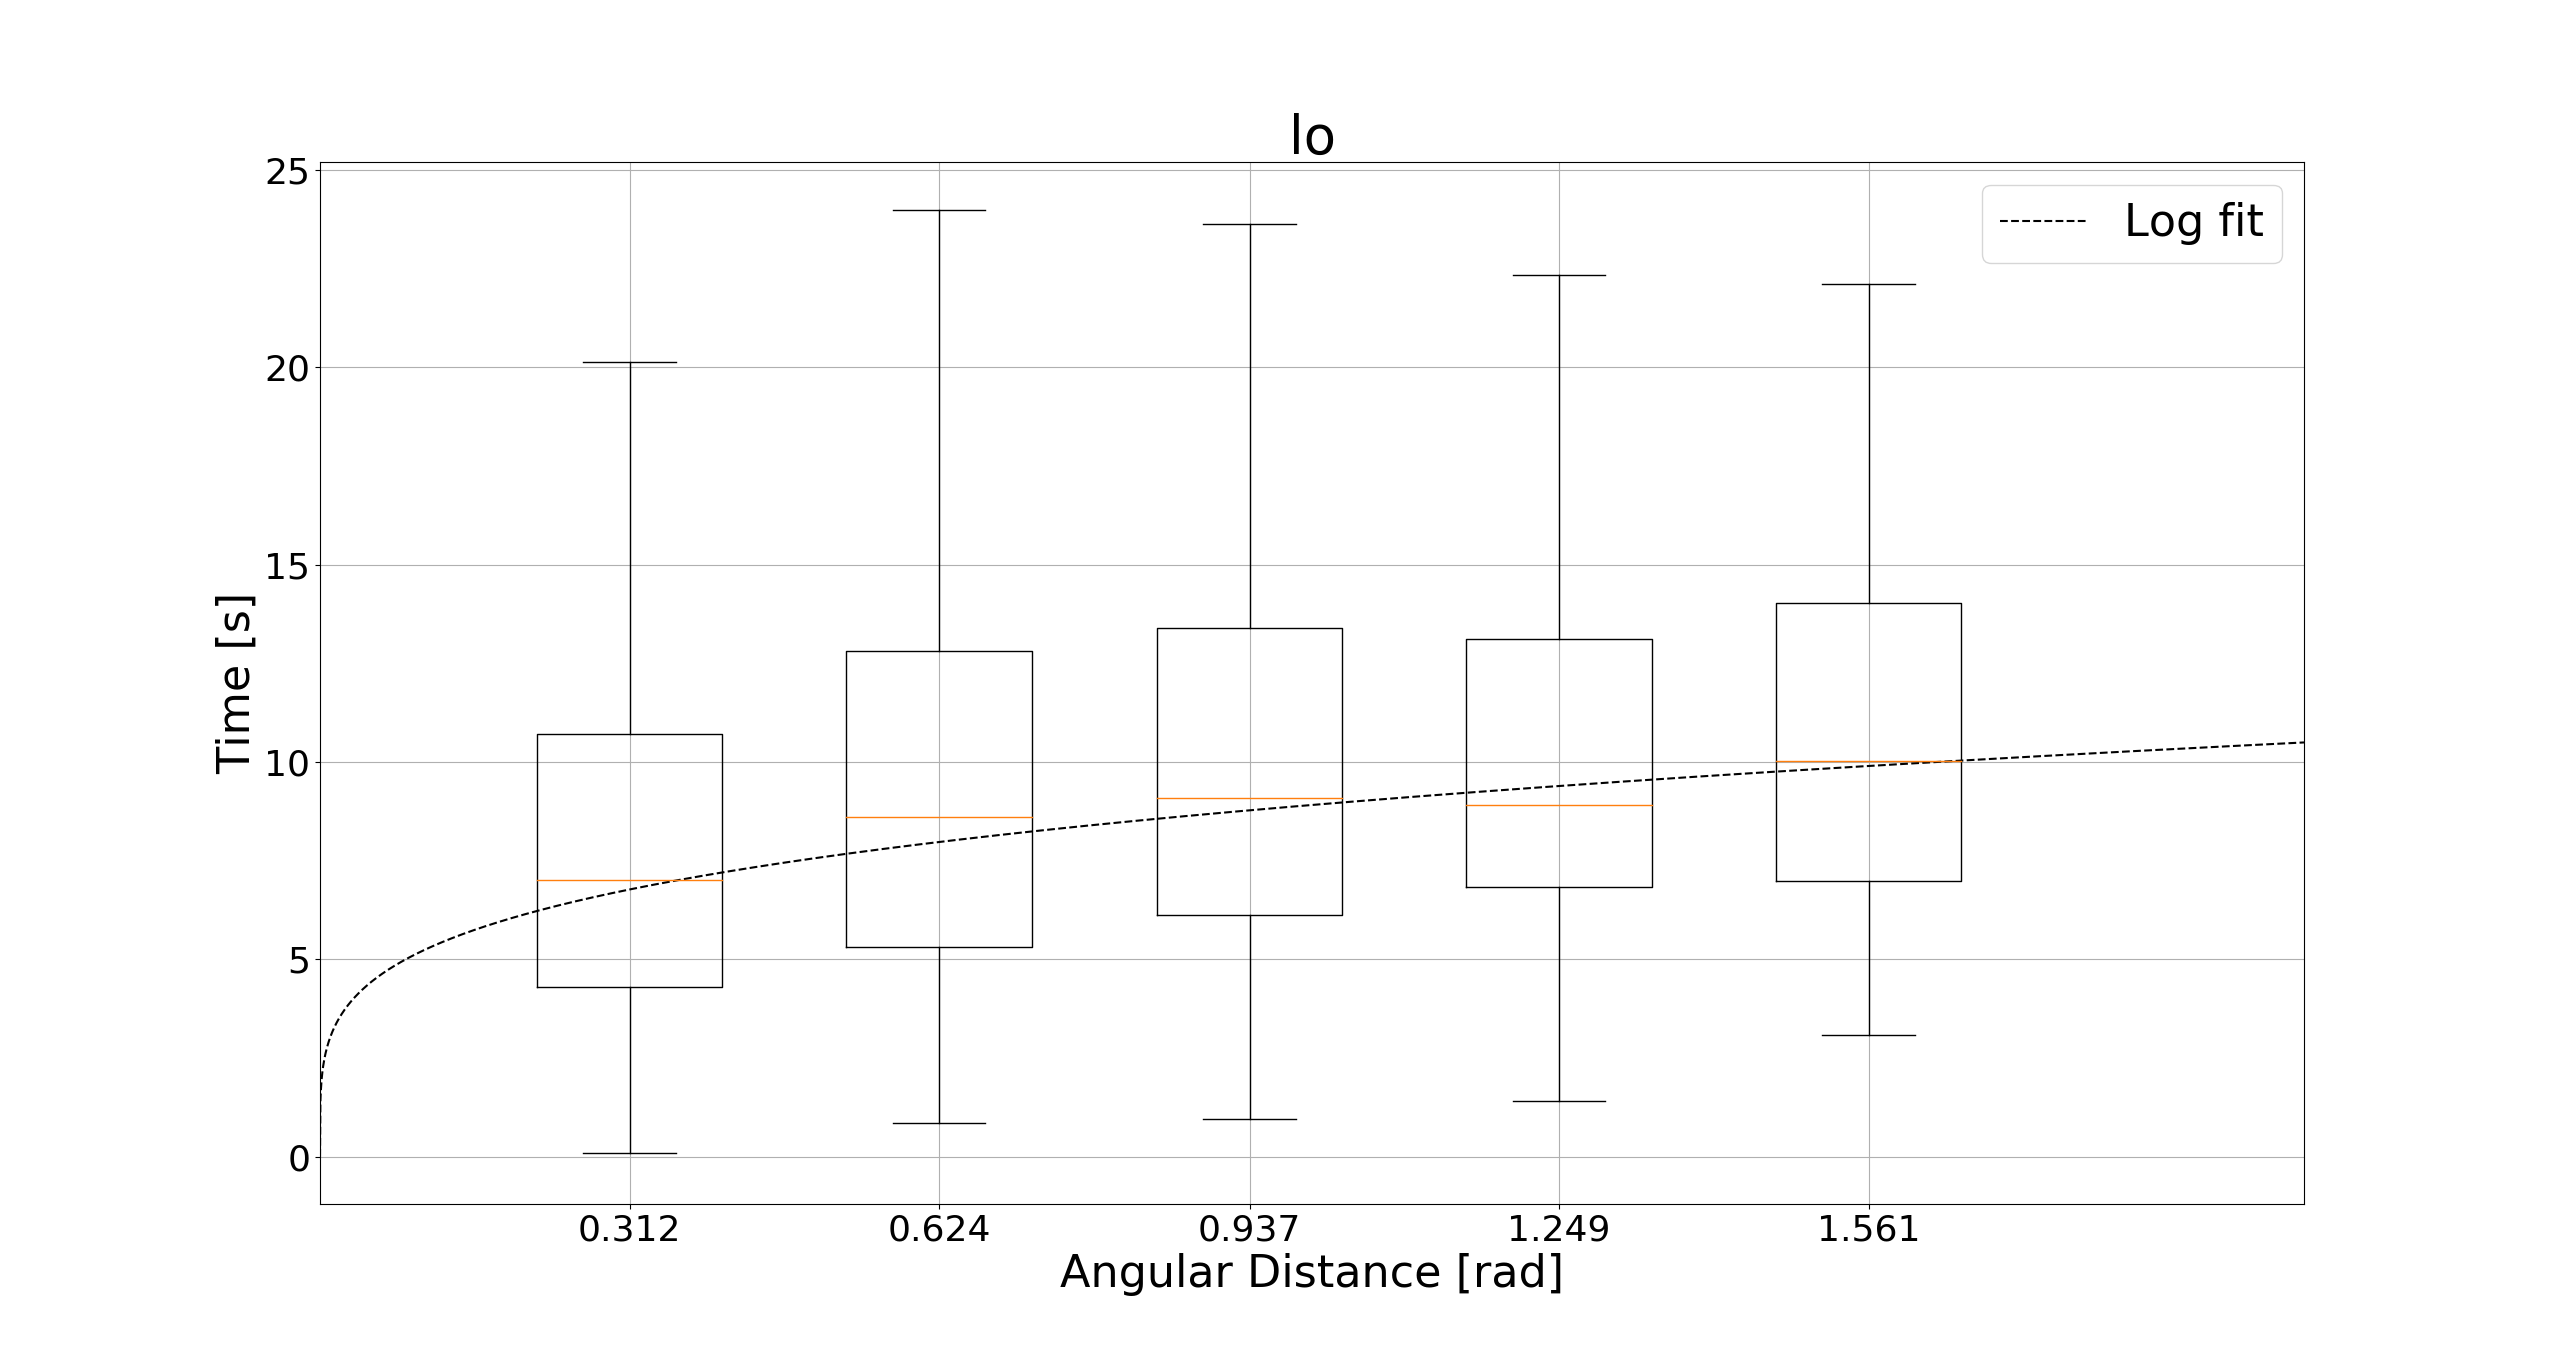
\includegraphics[width=0.5\textwidth]{figures/fitts_lo.png}
  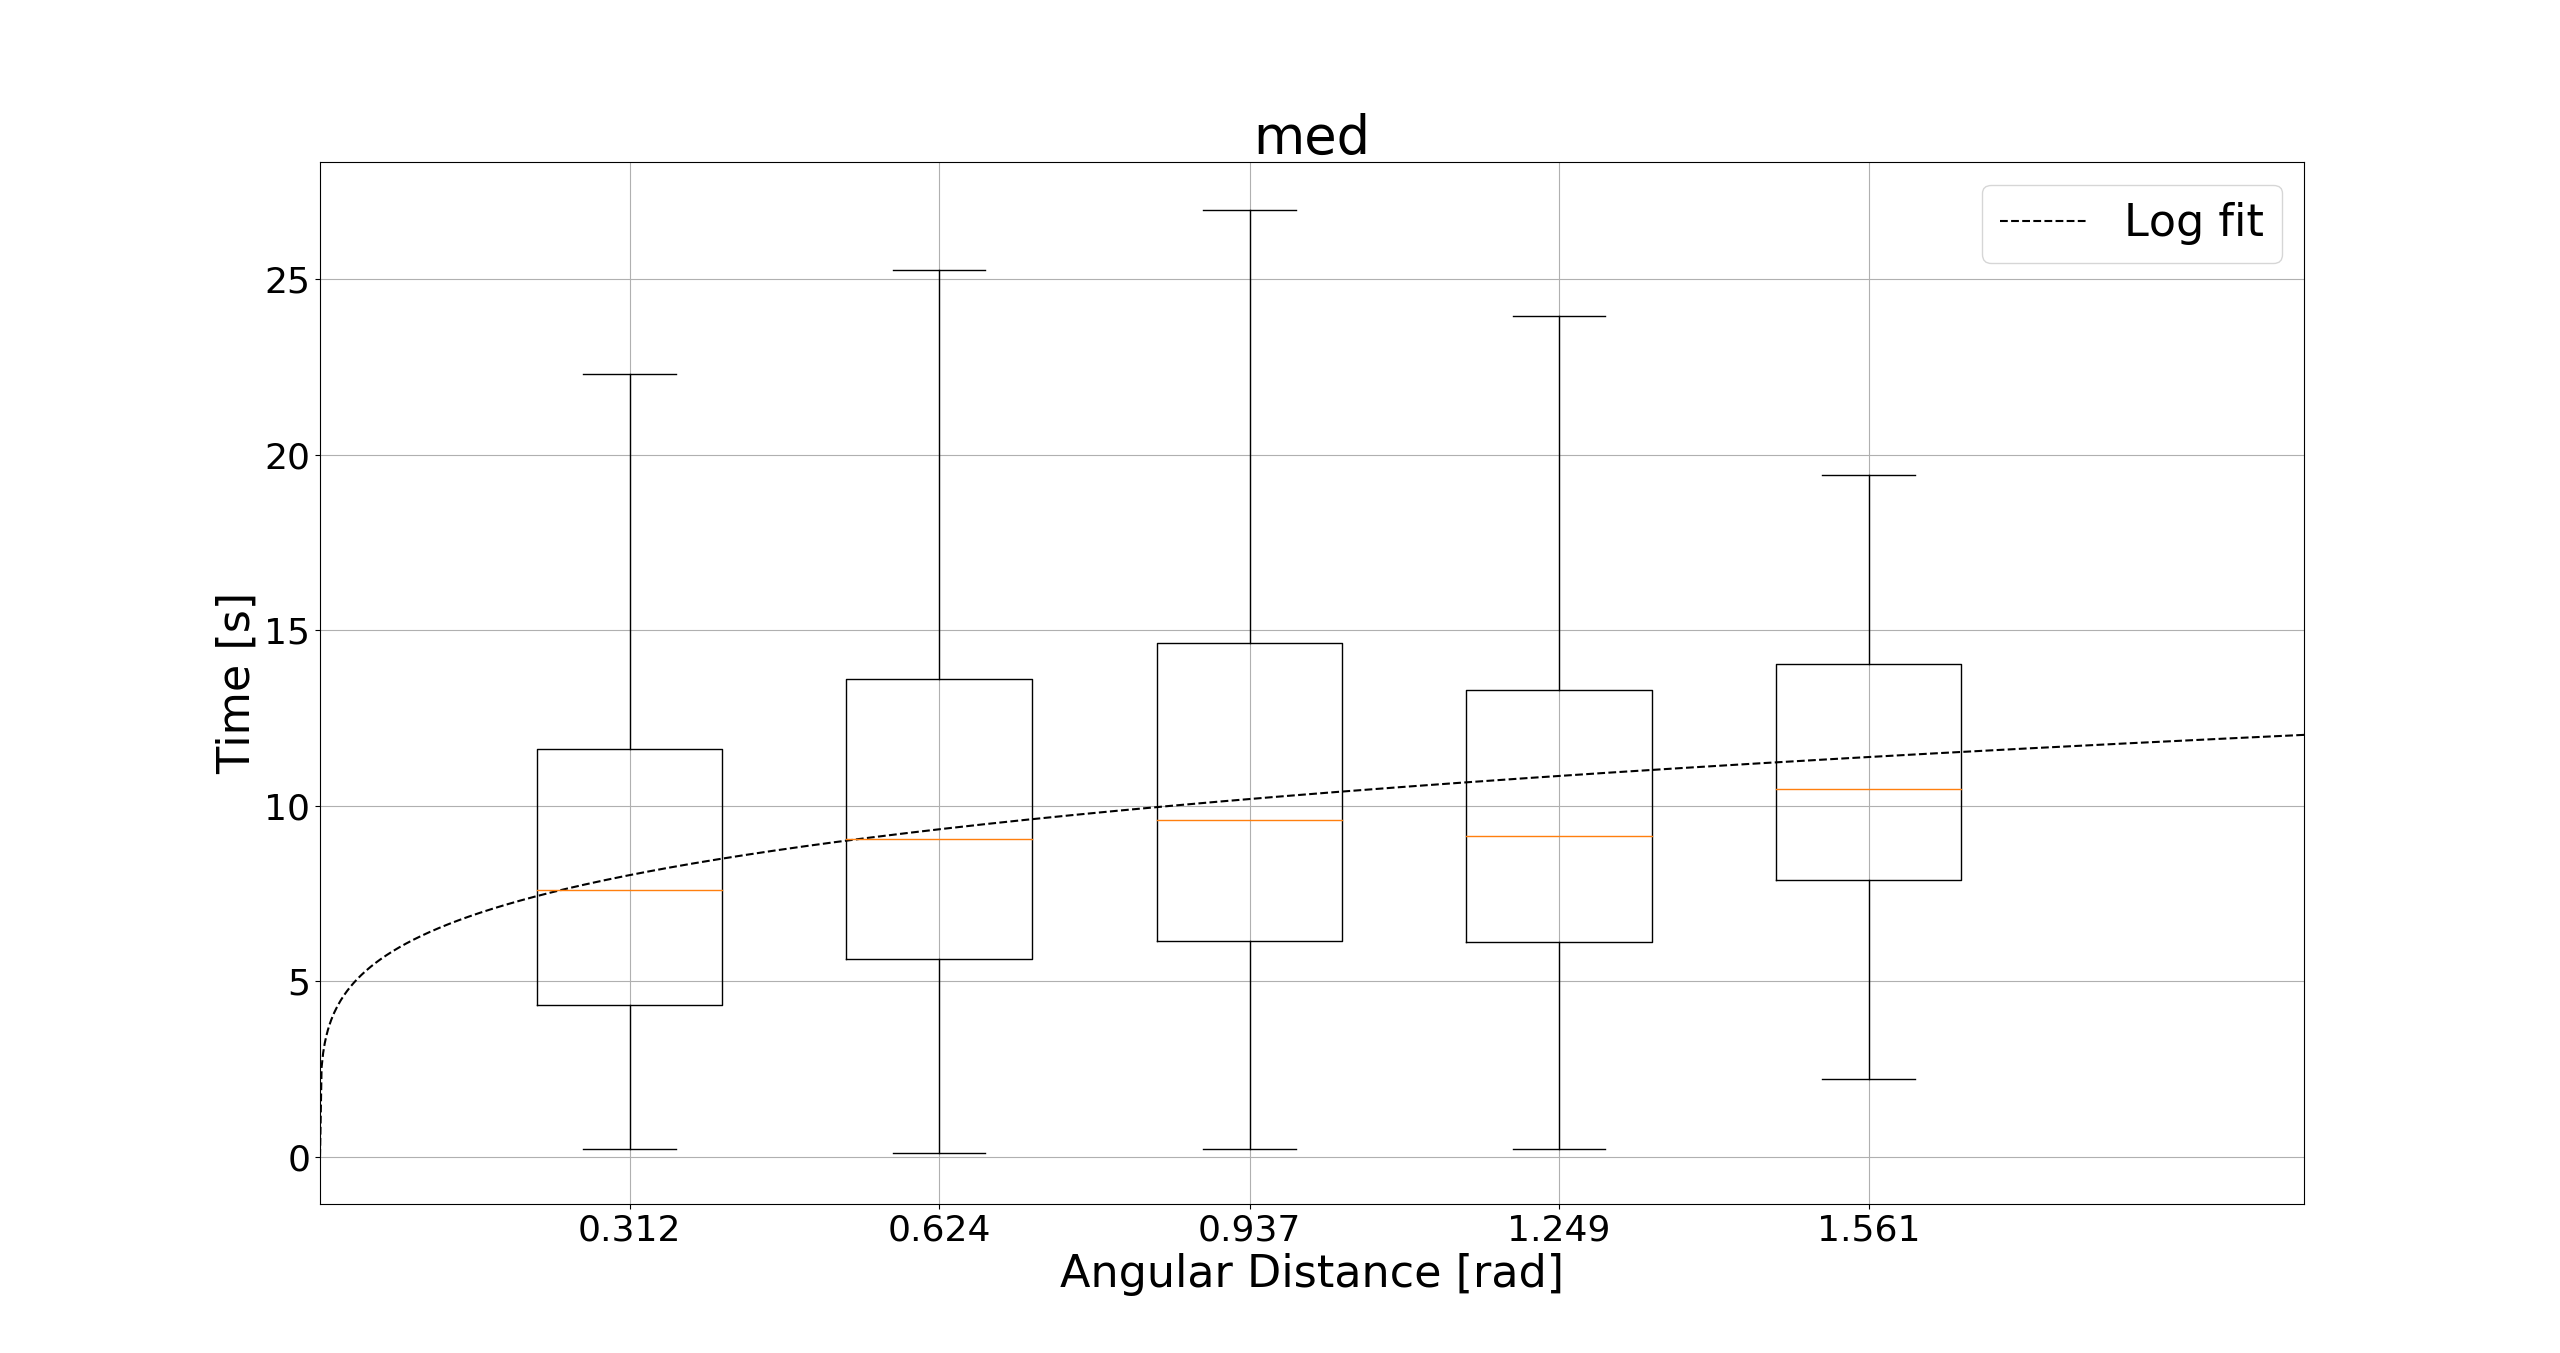
\includegraphics[width=0.5\textwidth]{figures/fitts_med.png}
  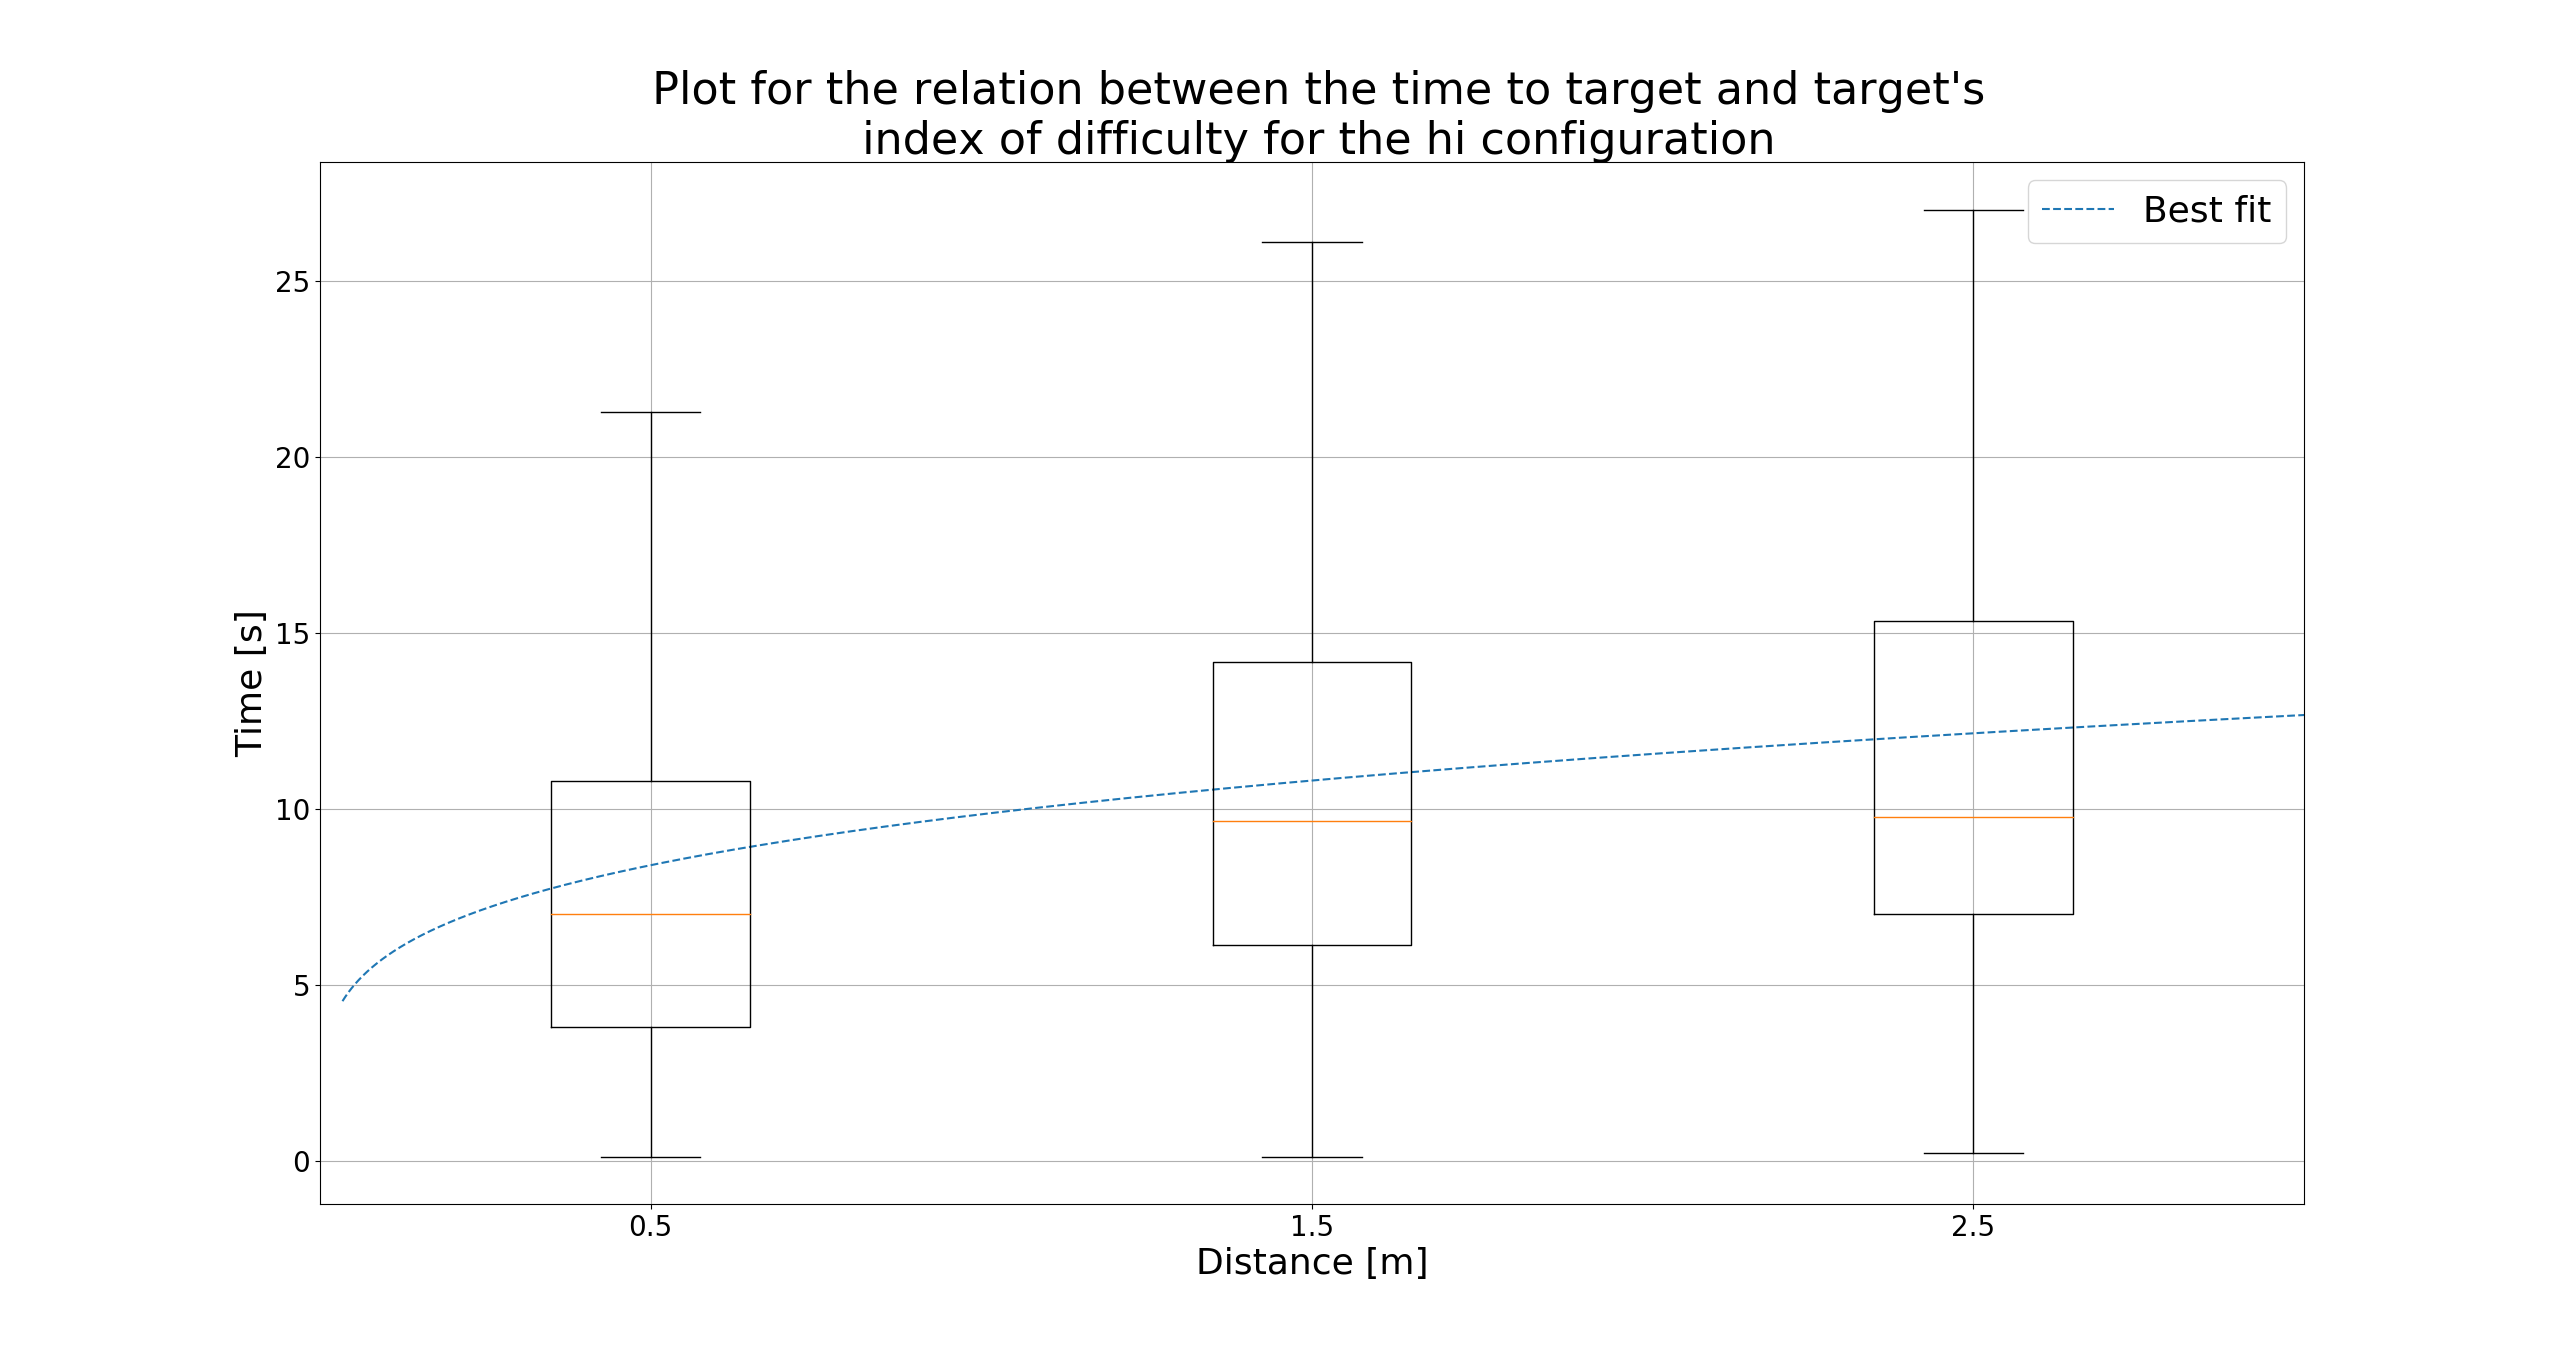
\includegraphics[width=0.5\textwidth]{figures/fitts_hi.png}
  \caption{The plots showing Fitts's Law relation between the targets' index of difficulty and the time it took the subjects to find the target. There is a plot for the \emph{lo}, \emph{med} and \emph{hi} pitch gain gradient configurations.} 
  \label{fig:fitts}
\end{figure}

From these figures we can see that the data roughly obeys Fitts's Law and forms a logarithmic graph. This enables us to use the index of performance, given by Equation~\ref{eq:fitts-performance}. We used this relation to plot Figure~\ref{fig:fitts-performance}.

\begin{figure}
  \centering
  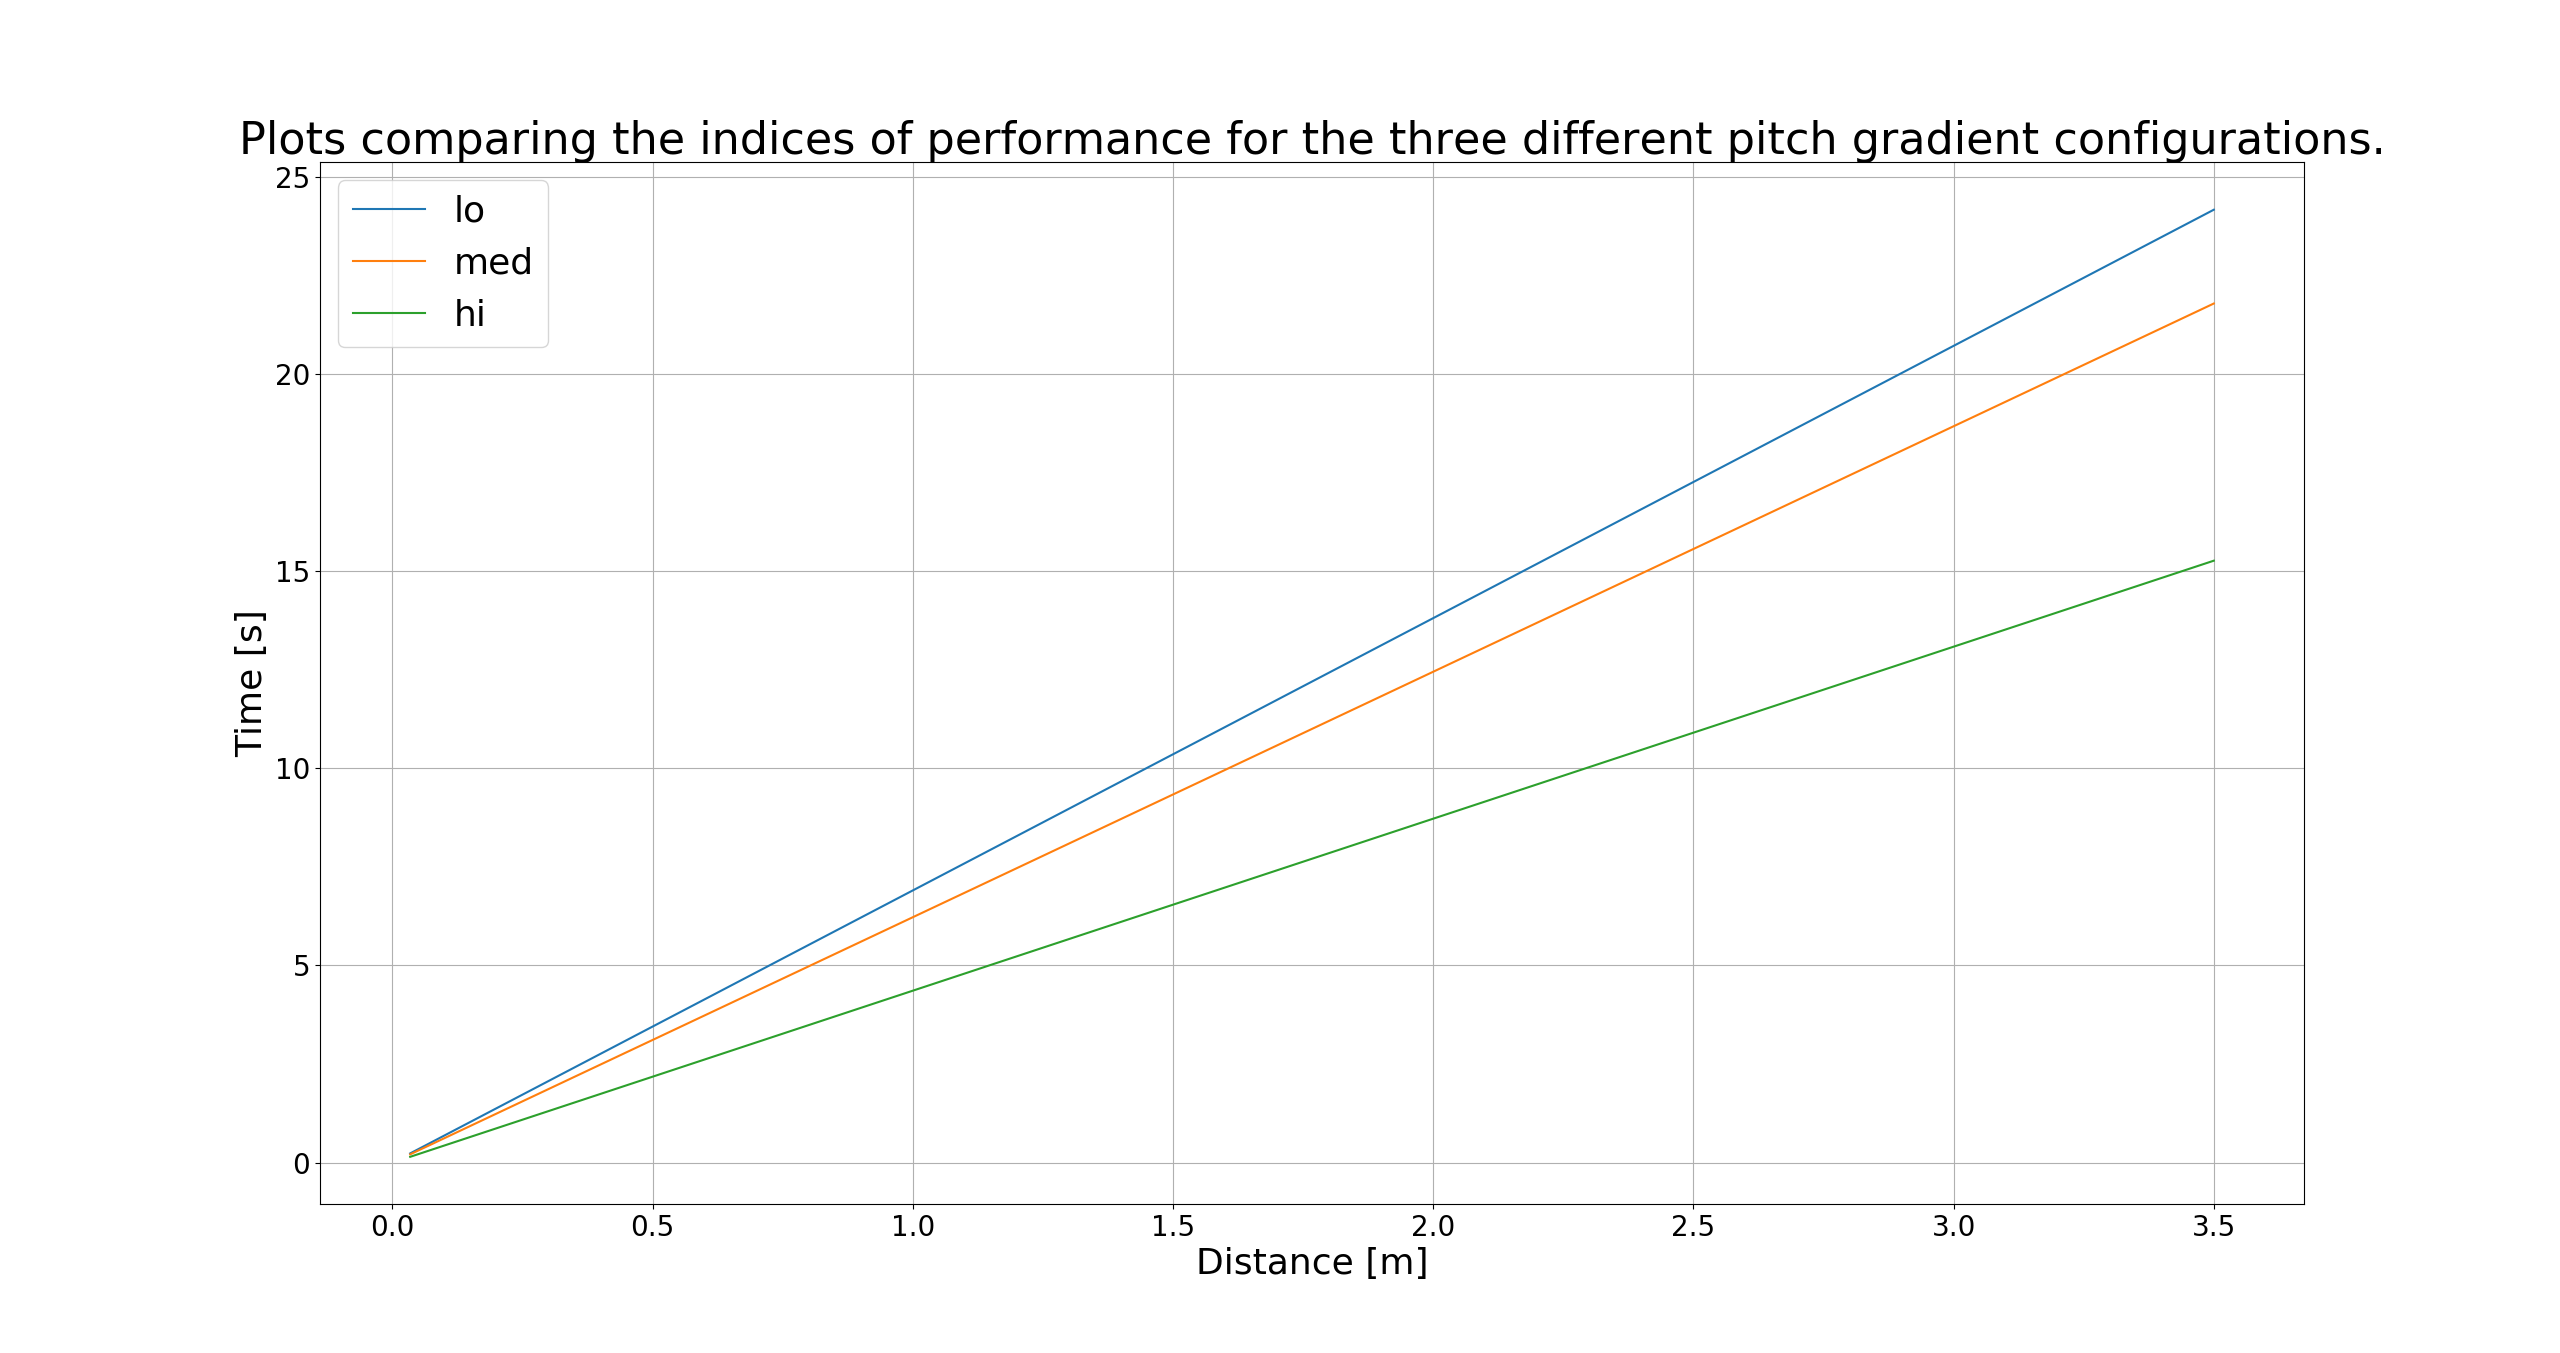
\includegraphics[width=0.5\textwidth]{figures/fitts_performance.png}
  \caption{A plot comparing the indices of performance for the three different pitch gradient configurations.}
  \label{fig:fitts-performance}
\end{figure}

From Figure~\ref{fig:fitts-performance} that the \emph{lo} and \emph{med} configurations give similar results with the \emph{hi} configuration gives the best result, where it took the average subject between 7 to 9 seconds less to find the most difficult target. 

\section{Conclusion and Future Work}
\label{sec:conclusion}

The next phase of the project is to add a co-adaptive module to the feedback interface, the goal of which is to refine the parameters of the feedback interface to better match the individual user's navigation habits and capability thereby increasing navigation performance and user satisfaction.

\section{Acknowledgements}
\label{sec:ack}

We would like to acknowledge and thank Google for their funding and support, as well as the UK's Engineering and Physical Sciences Research Council (EPSRC) and Visual Image Interpretation in Humans and Machines (ViiHM) for their funding and aid in carrying out these experiments. 

\bibliographystyle{ACM-Reference-Format}
\bibliography{icmi17}

\end{document}
